\documentclass{article}


\pdfinfoomitdate=1
\pdfsuppressptexinfo=15
\pdftrailerid{}



\usepackage{colm2024_conference}







\usepackage{graphicx}
\usepackage{float}
\usepackage{caption}
\usepackage[utf8]{inputenc} %
\usepackage[T1]{fontenc}    %
\usepackage{hyperref}       %
\usepackage{url}            %
\usepackage{booktabs}       %
\usepackage{amsfonts}       %
\usepackage{nicefrac}       %
\usepackage{microtype}      %
\usepackage{placeins}
\usepackage{xcolor}     %
\usepackage{colortbl}
\usepackage{wrapfig}
\usepackage{marvosym}

\makeatletter
\newcommand\blfootnote[1]{%
  \begingroup
  \renewcommand\thefootnote{}\footnote{#1}%
  \addtocounter{footnote}{-1}%
  \endgroup
}
\makeatother

\definecolor{darkred}{RGB}{177, 38, 26}
\definecolor{darkblue}{RGB}{67, 116, 177}
\definecolor{darkgreen}{rgb}{0.0, 0.5, 0.0}

\definecolor{bestcol}{RGB}{  0,102,204} %
\definecolor{goodcol}{RGB}{ 34,139, 34} %
\definecolor{deltaBg}{RGB}{220,230,255} %
\newcommand{\best}[1]{\textbf{\textcolor{bestcol}{#1}}}
\newcommand{\better}[1]{\textbf{\textcolor{goodcol}{#1}}}

\newcommand{\rowhighlight}{\rowcolor{deltaBg}}


\usepackage[inline]{enumitem}

\usepackage[most]{tcolorbox}
\usepackage{listings}
\usepackage{etoc}

\tcbset{
  colback=white, %
  colframe=black, %
  arc=2mm,            %
  boxrule=1pt,      %
  left=6pt, right=6pt, top=6pt, bottom=6pt  %
}


\usepackage{epigraph}
\setlength{\epigraphwidth}{0.85\linewidth}

\usepackage{amsmath, amssymb}
\usepackage[capitalize,noabbrev]{cleveref}

\usepackage{multirow}
\usepackage{array} 
\usepackage{tabularx}
\usetikzlibrary{calc}

\captionsetup[figure]{skip=4pt}

\newlist{inlinelist}{enumerate*}{1}
\setlist[inlinelist]{label=(\roman*)}

\newcommand{\shenzhi}[1] {{~\color{red}~[Shenzhi: #1]~}}

\newcommand{\CiteInline}[1]{\cite{#1}}
\newcommand{\CiteParen}[1]{\citep{#1}}

\makeatletter
\renewenvironment{abstract}{\vskip.075in\centerline{\large\bf Abstract}\vspace{0.5ex}\begin{quote}}{\par\end{quote}\vskip 1ex}
\makeatother



\title{HopChain: Multi-Hop Data Synthesis for Generalizable Vision-Language Reasoning}


\author{%
 \textbf{Shenzhi Wang$^{1,2,\ast}$, Shixuan Liu$^{1,\ast}$, Jing Zhou$^{1}$, Chang Gao$^{1}$, Xiong-Hui Chen$^{1}$, Binghai Wang$^{1}$, An Yang$^{1}$, Shiji Song$^{2}$, Bowen Yu$^{1,\textrm{\Letter},\dagger}$,  Gao Huang$^{2,\textrm{\Letter}}$, Junyang Lin$^{1}$} \\
 $^1$ Qwen Team, Alibaba Inc. \qquad $^2$ LeapLab, Tsinghua University
}



\begin{document}

\blfootnote{\hspace*{-1.5em}$^\ast$Equal contribution \quad $\textrm{\Letter}$: Corresponding authors \quad $\dagger$: Project lead}
\blfootnote{\hspace*{-1.5em}\mbox{\footnotesize Emails: \texttt{wangshenzhi99@gmail.com}, \texttt{liushixuan66@gmail.com}, \texttt{yubowen.ph@gmail.com}, \texttt{gaohuang@tsinghua.edu.cn}}}

\maketitle


\begin{abstract}
  Vision-language models (VLMs) show strong multimodal capabilities but still struggle with fine-grained vision-language reasoning.
We find that long chain-of-thought (CoT) reasoning exposes diverse failure modes, including perception, reasoning, knowledge, and hallucination errors, which can compound across intermediate steps.
However, most existing vision-language data used for reinforcement learning with verifiable rewards (RLVR) does not involve complex reasoning chains that rely on visual evidence throughout, leaving these weaknesses largely unexposed.
We therefore propose \textbf{HopChain}, a scalable framework for synthesizing \emph{multi-hop vision-language reasoning} data for RLVR training of VLMs.
Each synthesized multi-hop query forms a logically dependent chain of instance-grounded hops, where earlier hops establish the instances, sets, or conditions needed for later hops, while the final answer remains a specific, unambiguous number suitable for verifiable rewards.
We train Qwen3.5-35B-A3B and Qwen3.5-397B-A17B under two RLVR settings: the original data alone, and the original data plus HopChain's multi-hop data, and compare them across 24 benchmarks spanning STEM and Puzzle, General VQA, Text Recognition and Document Understanding, and Video Understanding.
Although this multi-hop data is not synthesized for any specific benchmark, it improves 20 of 24 benchmarks on both models, indicating broad and generalizable gains.
Consistently, replacing full chained queries with half-multi-hop or single-hop variants reduces the average score across five representative benchmarks from 70.4 to 66.7 and 64.3, respectively.
Notably, multi-hop gains peak in long-CoT vision-language reasoning, exceeding 50 points in the ultra-long-CoT regime.
These experiments establish HopChain as an effective, scalable framework for synthesizing multi-hop data that improves generalizable vision-language reasoning.

\end{abstract}

\section{Introduction} \label{sec: introduction}


\begin{figure}[!t]
  \centering
  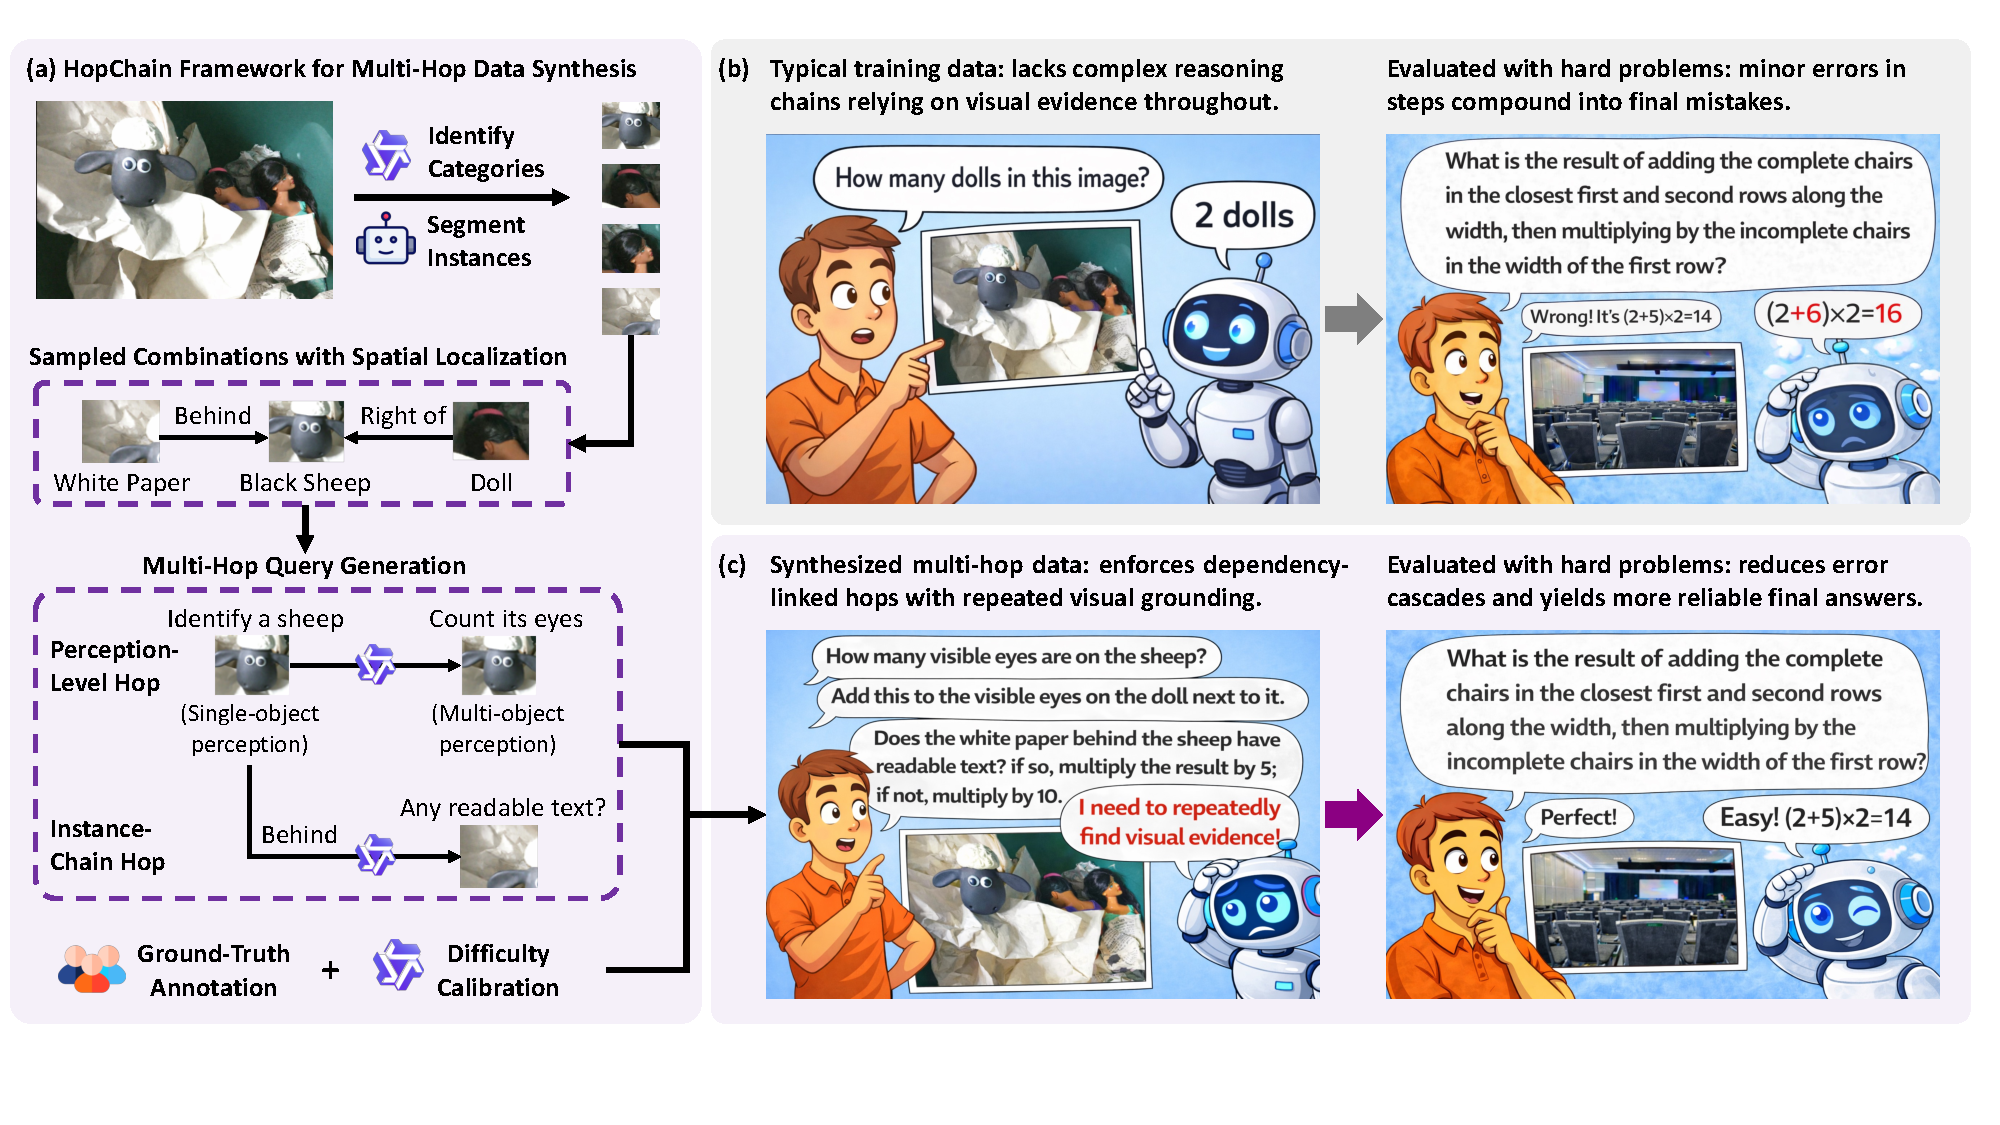
\includegraphics[width=1\textwidth]{imgs/teaser_multihop_4.pdf}
  \caption{Overview of HopChain and the motivation for multi-hop vision-language reasoning data. \textbf{(a)} HopChain synthesizes multi-hop data through four stages: category identification, instance segmentation, multi-hop query generation, and ground-truth annotation with difficulty calibration. \textbf{(b)} Typical vision-language training data often does not require complex reasoning chains that rely on visual evidence throughout; on hard problems, minor mistakes introduced at intermediate long-CoT steps can compound into final errors. \textbf{(c)} In contrast, the multi-hop data synthesized by HopChain forms logically dependent hop chains in which later hops depend on instances, sets, or conditions established by earlier hops, while nearly every hop requires fresh visual re-grounding. This training signal encourages continual visual evidence seeking during long-CoT reasoning, improving robustness and reducing compounding errors.}
  \label{fig:example_image}
  \vspace{-6pt}
\end{figure}

Vision-language models (VLMs) have achieved impressive performance across a diverse set of multimodal benchmarks by integrating visual encoders with large language models~\CiteParen{liu2024visual,liu2024improved,bai2023qwenvl,bai2025qwen25vl,chen2024internvl,openai2023gpt4,geminiteam2024gemini}.
Recent advances in reinforcement learning with verifiable rewards (RLVR) have further improved VLMs' reasoning abilities by training them to produce step-by-step chain-of-thought solutions for questions with objectively verifiable answers~\CiteParen{shao2024deepseekmath,deepseekr1}.
Despite this progress, a critical gap remains: VLMs frequently struggle with tasks that require \emph{fine-grained, multi-step vision-language reasoning}, where the correct answer depends on carefully attending to multiple visual elements and their relationships within an image~\CiteParen{bigverdi2025perception,ye2025blinktwice,jiang2025vlmr3}.


A natural question arises: \emph{what prevents current VLMs from performing robust vision-language reasoning?}
In \cref{sec: unreliable visual perception in long-chain reasoning}, we analyze a central challenge:
VLMs exhibit \textbf{diverse and compounding failure modes during long chain-of-thought (CoT) reasoning}, as longer reasoning chains may cause models to attend less faithfully to the image, execute incorrect intermediate reasoning steps, rely on incomplete knowledge, or produce hallucinated and weakly grounded intermediate content that then compounds across subsequent steps.
Related failure patterns have also been reported in prior analyses of amplified multimodal hallucination, evidential drift, object hallucination, visual illusion, and image-context reasoning errors~\CiteParen{liu2025morethinking,luo2025thinkingdrifts,rohrbach2018object,guan2024hallusionbench,leng2024vcd}.
Critically, as depicted in \cref{fig:example_image}(b), most existing vision-language training data does not involve particularly complex reasoning chains that depend on visual evidence throughout the process.
As a result, these long-CoT weaknesses remain largely unexposed during training.
This observation suggests that relying on, or simply expanding, existing vision-language RLVR training data is insufficient; what is needed is training data that \emph{structurally forces} the model to seek visual evidence at each step of long-CoT reasoning, strengthening step-by-step vision-language reasoning and improving generalization across diverse scenarios.


Motivated by this insight, we propose \textbf{HopChain}\footnote{Throughout this paper, HopChain refers to our synthesis framework, while \emph{multi-hop vision-language reasoning data}, or simply \emph{multi-hop data}, refers to the training data synthesized by HopChain.}, a scalable framework for synthesizing multi-hop vision-language reasoning data specifically for RLVR training of VLMs.
Each synthesized multi-hop query forms a logically dependent chain of instance-grounded hops, where earlier hops establish the instances, sets, or conditions needed for later hops, forcing repeated visual re-grounding throughout training rather than language-only shortcuts.
At the same time, each query terminates in a specific, unambiguous numerical answer that is easy to verify for RLVR; moreover, because the hops are logically dependent, obtaining the correct final number usually also requires the intermediate reasoning steps to be correct.
Rather than targeting a narrow synthetic task, we use the multi-hop data synthesized by HopChain as a complementary source of RLVR training data to strengthen fundamental vision-language reasoning under long CoT and support broad, generalizable gains across diverse domains.
Importantly, this synthesized data is not tailored to any particular downstream benchmark; instead, it is constructed to strengthen general-purpose vision-language reasoning, which we later show transfers broadly across benchmark families.
We define this multi-hop structure through two hop types: perception-level hops and instance-chain hops.
A \emph{perception-level hop} switches between single-object perception (e.g., read text, identify color, determine position) and multi-object relationship reasoning (e.g., compare sizes, count objects satisfying a condition, determine spatial arrangement), while remaining grounded in the instances, sets, or conditions established by earlier hops.
An \emph{instance-chain hop} follows an explicit dependency chain (e.g., instance A $\rightarrow$ B $\rightarrow$ C), where the next instance can be identified only from the instances, sets, or conditions established by earlier hops.
We require each query to combine both hop types in a logically dependent chain, where earlier hops establish the instances, sets, or conditions needed for later hops.
This design forces fresh visual grounding at every step, blocks language-only shortcuts, and exposes diverse long-CoT failure modes during training, as shown in \cref{fig:example_image}(c).

To construct such multi-hop data at scale, HopChain adopts a scalable four-stage data synthesis pipeline:
(1)~\emph{category identification} via Qwen3-VL-235B-A22B-Thinking~\CiteParen{qwen3vl2025} to enumerate semantic categories in each image;
(2)~\emph{instance segmentation} via SAM3~\CiteParen{carion2025sam3} to localize individual instances for the identified semantic categories;
(3)~\emph{multi-hop query generation} via Qwen3-VL-235B-A22B-Thinking that constructs logically chained questions over combinations of instances; and
(4)~\emph{human-in-the-loop verification} where multiple annotators independently solve each query, and only queries with the same final numerical answer are retained as valid training examples.
The pipeline provides a scalable data synthesis workflow, scaling to broad image collections with sufficient detectable instances while maintaining strict quality control, as summarized in \cref{fig:example_image}(a).

We apply RLVR with Soft Adaptive Policy Optimization (SAPO)~\CiteParen{sapo} on the multi-hop data synthesized by HopChain to train VLMs.
We validate the effectiveness of the multi-hop data synthesized by HopChain on Qwen3.5-35B-A3B and Qwen3.5-397B-A17B~\CiteParen{qwen35blog} across 24 benchmarks spanning STEM and Puzzle, General VQA, Text Recognition and Document Understanding, and Video Understanding.
Compared with RLVR on the original RLVR data alone, adding this multi-hop data improves 20 out of 24 benchmarks on both Qwen3.5-35B-A3B and Qwen3.5-397B-A17B, despite the fact that the synthesized data is not designed for any specific benchmark, indicating broad and generalizable performance gains across diverse scenarios.
To demonstrate that full chained queries are important, we replace them with half-multi-hop or single-hop variants on Qwen3.5-35B-A3B, reducing the average score across five representative benchmarks from 70.4 to 66.7 and 64.3, respectively.
Multi-hop training substantially strengthens long-CoT vision-language reasoning, with gains peaking at more than 50 accuracy points in the ultra-long-CoT regime on Qwen3.5-397B-A17B.
When we independently sample each synthesized query multiple times on both Qwen3.5-35B-A3B and Qwen3.5-397B-A17B, more than half of the queries are partially solved and the outcomes are distributed relatively evenly from fully incorrect to fully correct, indicating a broad difficulty range suitable for both smaller and larger models. The corrected error types also closely follow the original error distribution before adding this multi-hop data, indicating gains that are broad rather than confined to a single narrow failure mode.
These extensive experiments establish HopChain as an effective framework for synthesizing multi-hop data that improves generalizable vision-language reasoning capabilities beyond the synthesized training distribution.

\vspace{0.3em}
\noindent Our main contributions are as follows:
\begin{itemize}[leftmargin=1.5em, itemsep=2pt, topsep=2pt]
    \item We identify diverse and compounding failure modes during long CoT reasoning as a key barrier to vision-language generalization, and show why relying on or simply expanding existing vision-language RLVR training data is insufficient.
    \item We formalize multi-hop vision-language reasoning with perception-level and instance-chain hops, and build HopChain, a scalable synthesis pipeline whose queries form logically dependent chains in which earlier hops establish the instances, sets, or conditions needed for later hops, forcing repeated visual re-grounding throughout training while keeping the final answer directly verifiable for RLVR.
    \item Through extensive experiments, we verify that RLVR on the multi-hop data synthesized by HopChain yields broad, generalizable gains: 20 out of 24 benchmarks improve on both Qwen3.5-35B-A3B and Qwen3.5-397B-A17B, while additional analyses show that preserving full chained queries is important, multi-hop data strengthens long-CoT vision-language reasoning, and the synthesized data spans a broad difficulty range while enabling trained models to correct a broad range of errors.
\end{itemize}


\section{Preliminaries}




\subsection{Reinforcement Learning with Verifiable Rewards for Vision-Language Models}

The reinforcement learning with verifiable rewards (RLVR) framework for vision-language models (VLMs) closely parallels that for large language models (LLMs), with the primary distinction being that RLVR for VLMs processes both an image and a text query as input to generate a textual chain-of-thought culminating in a verifiable answer prediction, whereas RLVR for LLMs operates solely on text queries.
Specifically, RLVR for VLMs aims to maximize the following objective:
\begin{align}
    &J(\pi) = \mathbb{E}_{(\boldsymbol{I}, \boldsymbol{q}, \boldsymbol{a}) \sim \mathcal{D}, \boldsymbol{o} \sim \pi(\cdot \mid \boldsymbol{I}, \boldsymbol{q})}[R(\boldsymbol{o}, \boldsymbol{a})],
    \\
    \text{where} & \quad  R(\boldsymbol{o}, \boldsymbol{a}) = \begin{cases} 1.0 & \text{if}\ \texttt{is\_equivalent}(\boldsymbol{o}, \boldsymbol{a}), \\ 0.0 & \text{otherwise.} \end{cases} \label{eq: reward calculation}
\end{align}
Here, $\boldsymbol{I}$, $\boldsymbol{q}$, and $\boldsymbol{a}$ denote the image, text query, and ground-truth answer, respectively, sampled from dataset $\mathcal{D}$, and $\boldsymbol{o}$ represents the response generated by policy $\pi$ conditioned on $\boldsymbol{I}$ and $\boldsymbol{q}$.




\subsection{Soft Adaptive Policy Optimization}

Soft Adaptive Policy Optimization (SAPO, \CiteParen{sapo}) is introduced to mitigate the potential instability and inefficiency caused by hard clipping in prior RLVR algorithms such as GSPO~\CiteParen{gspo} and GRPO~\CiteParen{shao2024deepseekmath}.
Concretely, SAPO substitutes hard clipping with a temperature-controlled soft gate and optimizes the following objective for VLMs:
\begin{equation}
\mathcal{J}(\theta)
=
\mathbb{E}_{(\boldsymbol{I}, \boldsymbol{q}, \boldsymbol{a}) \sim \mathcal{D}, \{\boldsymbol{o}_i\}_{i=1}^G \sim \pi_{\text{old}}(\cdot \mid \boldsymbol{I}, \boldsymbol{q})}
\left[
\frac{1}{G}
\sum_{i=1}^{G}
\frac{1}{|\boldsymbol{o}_i|}
\sum_{t=1}^{|\boldsymbol{o}_i|}
f_{i,t}\!\left(r_{i,t}(\theta)\right)
\hat{A}_{i,t}
\right],
\end{equation}
\begin{align}
\text{where} \quad &r_{i,t}(\theta)
=
\frac{
\pi_{\theta}\!\left(\boldsymbol{o}_{i,t} \mid \boldsymbol{I}, \boldsymbol{q}, \boldsymbol{o}_{i,<t}\right)
}{
\pi_{\theta_{\text{old}}}\!\left(\boldsymbol{o}_{i,t} \mid \boldsymbol{I}, \boldsymbol{q}, \boldsymbol{o}_{i,<t}\right)
},
\qquad
\hat{A}_{i,t}
=
\hat{A}_i
=
\frac{
R_i - \operatorname{mean}\!\left(\{R_j\}_{j=1}^{G}\right)
}{
\operatorname{std}\!\left(\{R_j\}_{j=1}^{G}\right)
},
\\
&f_{i,t}(x)
=
\sigma\!\left(\tau_{i,t}(x - 1)\right)
\cdot
\frac{4}{\tau_{i,t}},
\qquad
\tau_{i,t}
=
\begin{cases}
\tau_{\text{pos}}, & \text{if } \hat{A}_{i,t} > 0, \\
\tau_{\text{neg}}, & \text{otherwise}.
\end{cases}
\end{align}
Here, $i, j$ denote the sample indices in $\mathcal{D}$, and $t$ is the token index within a sequence. 
The parameters of the currently trained policy and the old rollout policy are denoted by $\theta$ and $\theta_{\text{old}}$, respectively. 
The temperatures for positive and negative tokens are $\tau_{\text{pos}}$ and $\tau_{\text{neg}}$, respectively. 
Moreover, $R_i$ is computed according to \cref{eq: reward calculation} for the $i$-th sample, and $\sigma(x) = \frac{1}{1 + e^{-x}}$ denotes the sigmoid function.


\section{Diverse Failure Modes in Long Chain-of-Thought Reasoning} \label{sec: unreliable visual perception in long-chain reasoning}

\begin{figure}[t]
    \centering
    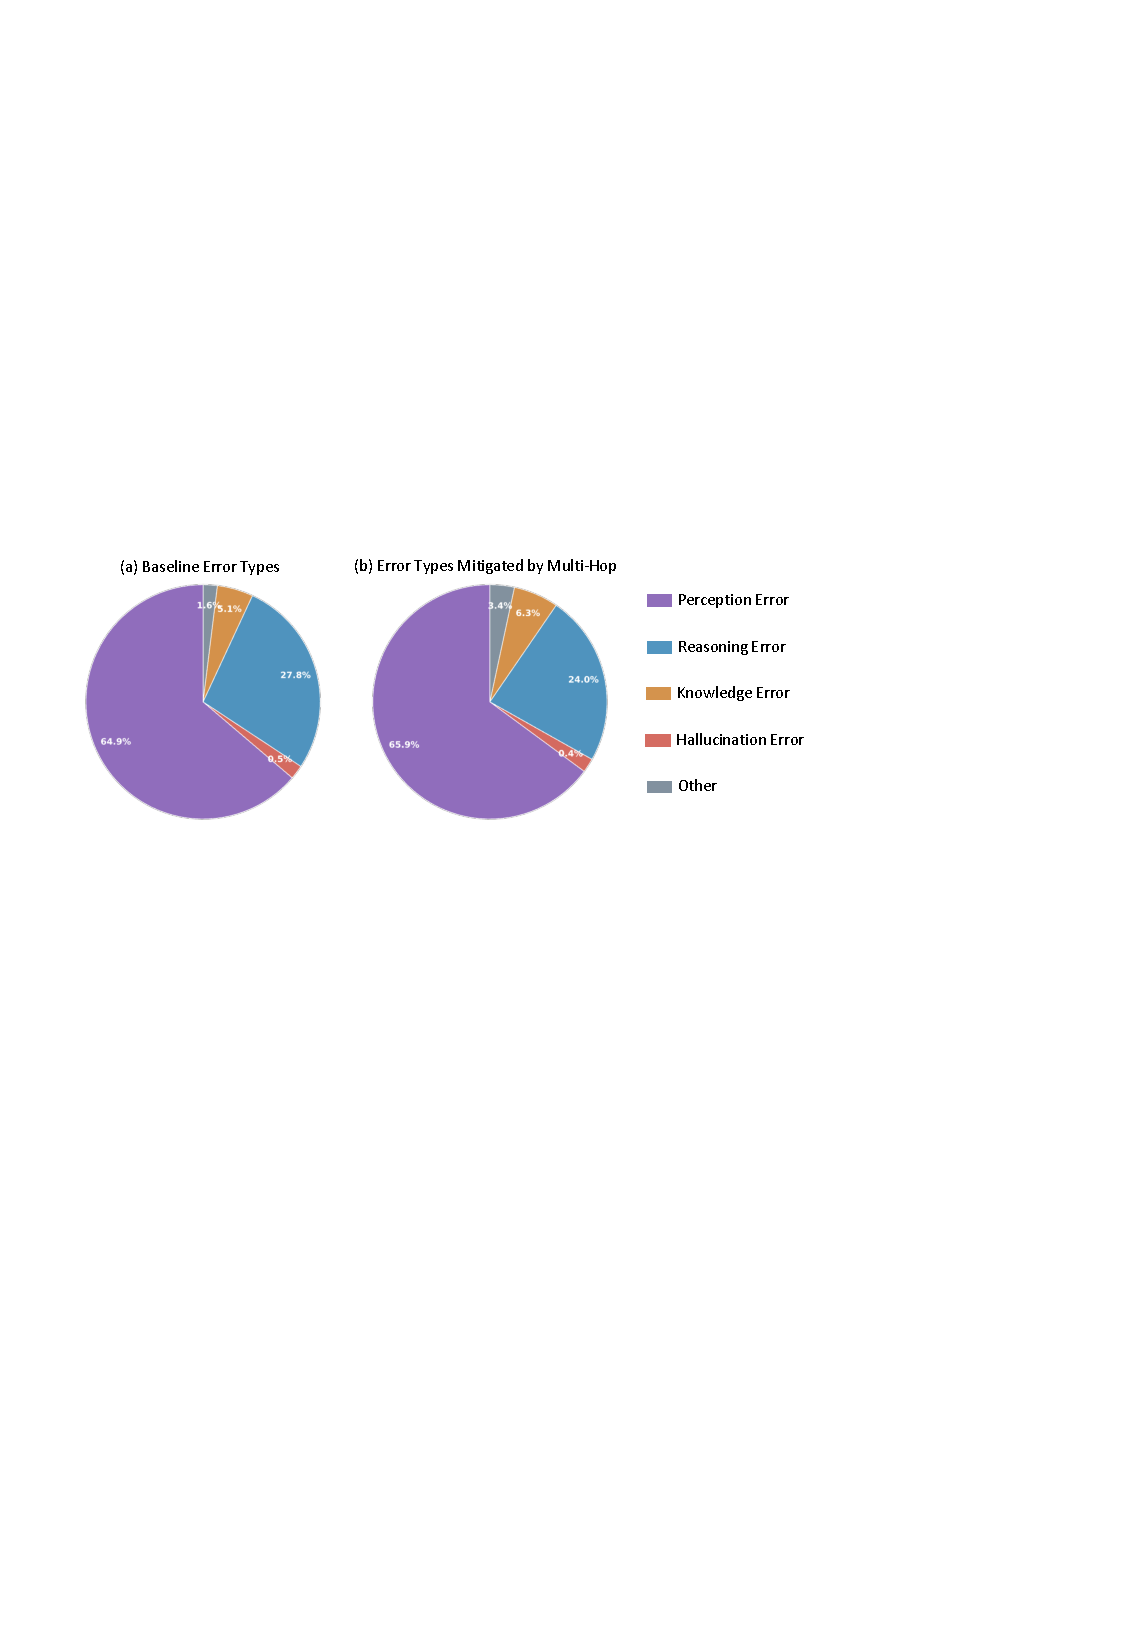
\includegraphics[pagebox=cropbox,width=0.8\textwidth]{imgs/error_distribution_new_2.pdf}
    \caption{Error-type distributions before and after adding multi-hop data in RLVR. Subfigure (a) shows the error-type distribution of \texttt{RLVR w/o Multi-Hop} on the benchmarks in Tables~\ref{tab:exp-35b} and~\ref{tab:exp-397b}. Subfigure (b) shows the distribution of baseline error types mitigated after adding multi-hop data (i.e., cases corrected by \texttt{RLVR w/ Multi-Hop}). In (a), errors are diverse, with perception and reasoning errors as the dominant categories. In (b), the distribution remains similar to (a), indicating that multi-hop data mitigates failures in a generalizable way rather than improving only a narrow error type. \Cref{fig:qualitative_examples} provides representative perception reasoning failures, together with responses corrected after adding multi-hop data.}
    \label{fig:error_distribution}
\end{figure}

Long CoT reasoning places a much higher demand on visual grounding than short, single-step QA.
To answer correctly, a VLM must repeatedly return to the image, recover the right object, attribute, relation, or numeric evidence at each step, and use that evidence to determine the next step of reasoning.
This makes long CoT reasoning inherently fragile: multiple error types can emerge along the chain, including perception, reasoning, knowledge, and hallucination errors, among others.
Once any such error appears at an intermediate step, the remaining reasoning can still look coherent while operating on flawed intermediate evidence, eventually producing an incorrect final answer.
Recent analyses in multimodal reasoning report similar patterns: longer reasoning traces can drift away from image-grounded evidence, reduce attention to visual inputs, and amplify hallucinated intermediate content~\CiteParen{liu2025morethinking,luo2025thinkingdrifts}.
More generally, diagnostic studies of VLMs have also documented persistent object hallucination and visual illusion under image-context reasoning~\CiteParen{rohrbach2018object,guan2024hallusionbench}.



\begin{figure}[!h]
    \centering
    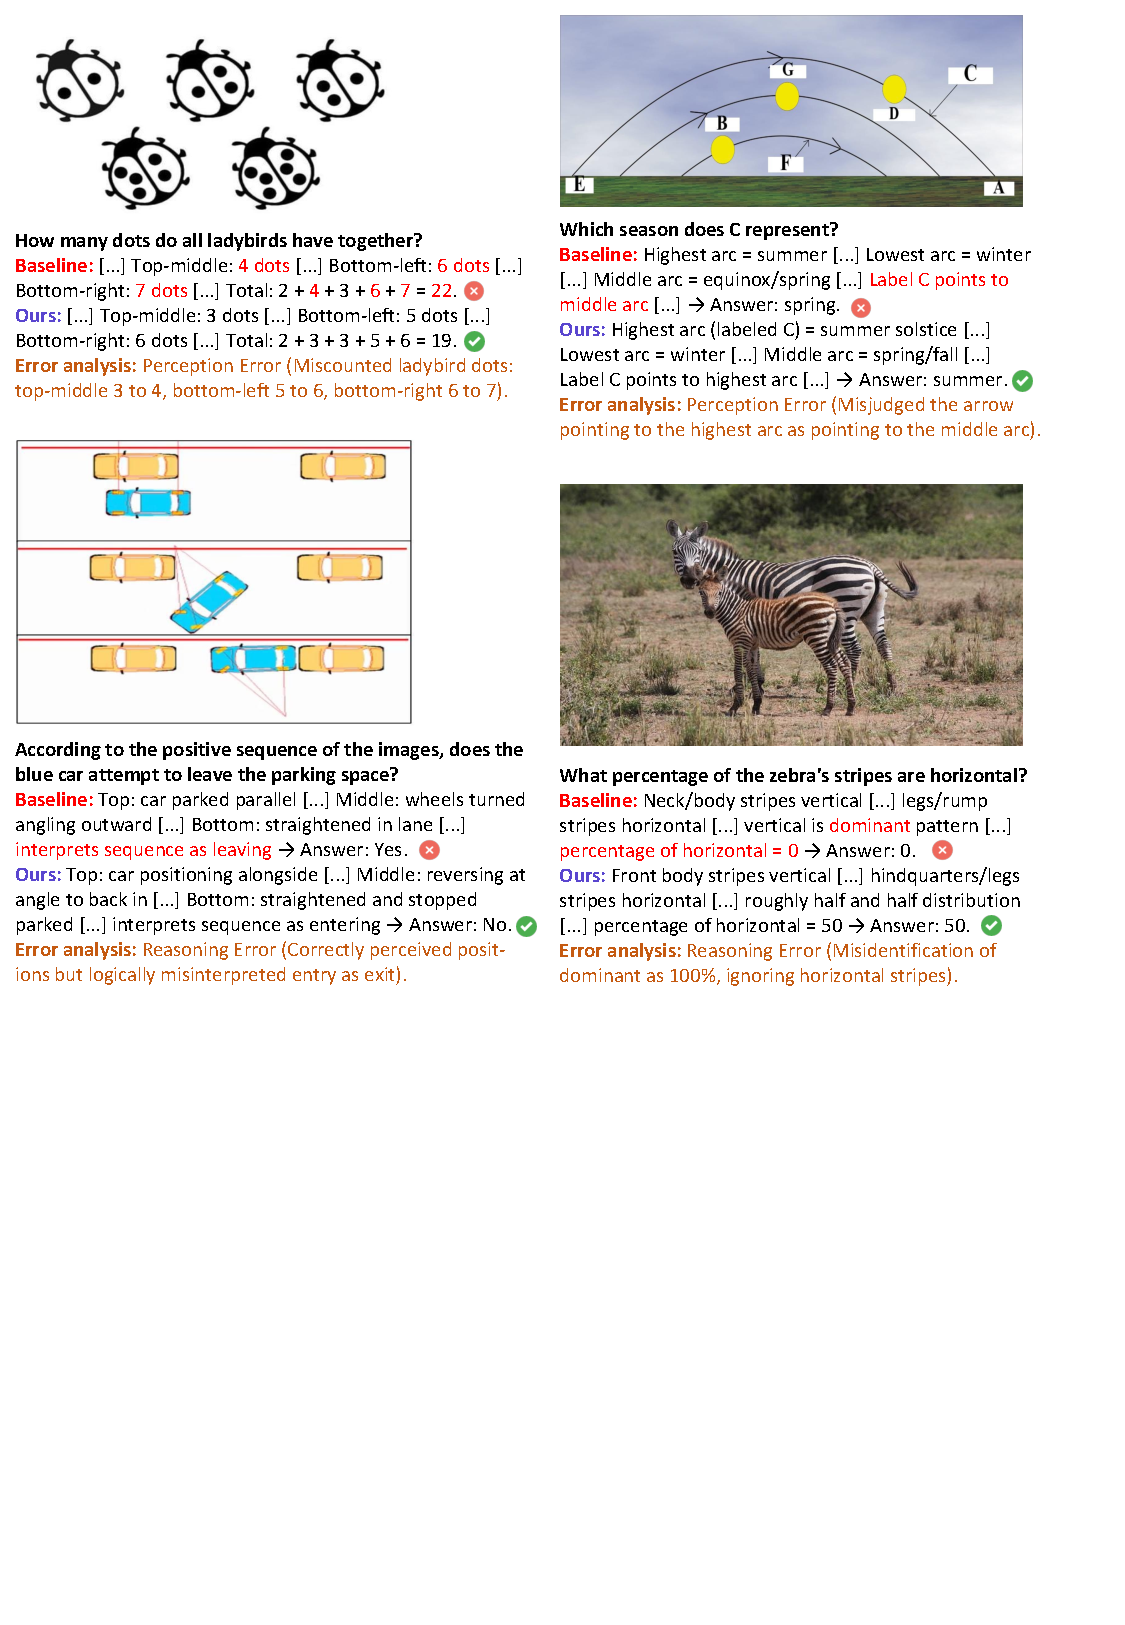
\includegraphics[width=1\textwidth]{imgs/qualitative_examples_new_5.pdf}
    \caption{Qualitative examples of unreliable visual perception in long CoT reasoning. We show failure cases from the benchmarks in \cref{tab:exp-35b,tab:exp-397b} using ``RVLR w/o Multi-Hop'' (baseline), alongside correct answers from ``RVLR w/ Multi-Hop'' (ours). For brevity, unimportant parts of the long CoT are omitted with $[\dots]$. The baseline error is highlighted in red, and the failure reason is given in the error analysis.}
    \label{fig:qualitative_examples}
    \vspace{-5pt}
\end{figure}


To obtain the error breakdown in \cref{fig:error_distribution}, we analyze responses produced on the benchmarks in \cref{tab:exp-397b} by Qwen3.5-397B-A17B under the \texttt{RLVR w/o Multi-Hop} setting. For each benchmark, we randomly sample 20 incorrect responses and ask annotators to identify the primary failure type by comparing the model output against the ground-truth answer.
The resulting breakdown shows that long-CoT failures are diverse rather than concentrated in a single category: perception errors are the largest group, while reasoning, knowledge, and hallucination errors are also present in the breakdown.
Qualitative examples in \cref{fig:qualitative_examples} further show that these failures are not limited to a narrow benchmark type.
The baseline model (\texttt{RLVR w/o Multi-Hop}) miscounts small local details in the ladybird example, misjudges the contact relation between the gripper and the dress strap, misreads the sign shape in the driving scene, reads chart values incorrectly, follows the wrong arc in the astronomy diagram, and selects the wrong body part in the fish illustration.
These examples cover natural images, charts, and scientific diagrams, but they share the same structure: one faulty intermediate step appears in the middle of a long reasoning chain, and the later reasoning steps inherit that mistake.
In this sense, long-CoT errors are often coupled rather than isolated: a mistaken visual judgment can trigger faulty reasoning, unsupported inference, or other downstream failures.
By contrast, \texttt{RLVR w/ Multi-Hop} is more likely to recover the correct visual evidence at each hop and therefore reaches the correct final prediction.

This analysis suggests that the central challenge is not merely producing a longer textual CoT, but maintaining reliable, step-wise reasoning over visual evidence throughout the chain across diverse visual scenarios.
This interpretation is also aligned with recent work arguing that multimodal reasoning is often bottlenecked by perception quality and can benefit from stronger intermediate perception, repeated image-grounded observation, or iterative revisiting of visual regions~\CiteParen{bigverdi2025perception,ye2025blinktwice,jiang2025vlmr3}.
Consequently, improving long CoT reasoning requires an RLVR data construction method that is applicable to diverse images, forces repeated grounding during reasoning, and trains the model to use the result of one step to locate, verify, or constrain the next.
This is exactly the goal of the HopChain framework introduced in the next section.



















































































\section{Boosting Vision-Language Generalization by Synthesizing Multi-Hop Data}
\label{sec: method}

The analysis in \cref{sec: unreliable visual perception in long-chain reasoning} shows that long-CoT reasoning does not fail for a single reason: models may make perception, reasoning, knowledge, hallucination, and other errors, and these errors often propagate once an incorrect intermediate step is carried forward through the rest of the chain.
This motivates training data beyond simply relying on, or expanding, existing vision-language RLVR training data. Specifically, the desired training data should structurally force the model to seek visual evidence at each step of long-CoT reasoning, thereby strengthening step-by-step vision-language reasoning and improving generalization across diverse scenarios.
Accordingly, we synthesize multi-hop vision-language reasoning data whose hops are designed to instantiate exactly this requirement, while ensuring that each query terminates in a specific, unambiguous numerical answer compatible with RLVR, as illustrated in \cref{fig:multihop-query-examples}.

\subsection{Multi-Hop Vision-Language Reasoning Definition}
\label{subsec:mh-vl-definition}

We first define the structure of the target multi-hop queries. To do so, we use three reasoning levels: Levels~1 and~2 describe what an individual reasoning step asks the model to do, while Level~3 describes a query that chains multiple Level~1 and Level~2 steps together.
\textbf{Level~1} is single-object perception, such as reading text or identifying object attributes, including color, shape, size, position, and category.
\textbf{Level~2} is multi-object perception, such as spatial, comparative, or counting relations across objects.
\textbf{Level~3} is multi-hop reasoning, where multiple Level~1 and Level~2 steps are chained into one query.

Within such a Level~3 query, consecutive hops can be linked in two complementary dimensions.
\textbf{Perception-level hop:} the next step changes the kind of perception being performed, for example from a Level~1 single-object judgment to a Level~2 relational judgment, or vice versa, while remaining grounded in the instances, sets, or conditions established by earlier hops.
\textbf{Instance-chain hop:} the next step moves to a new instance along an explicit dependency chain (e.g., instance A $\rightarrow$ B $\rightarrow$ C), where the next instance can only be identified from the instances, sets, or conditions established by earlier hops.

Each query must satisfy three structural conditions: (\romannumeral1) it must be Level~3, (\romannumeral2) it must combine both hop types, and (\romannumeral3) its hops must form a logically dependent chain in which earlier hops establish the instances, sets, or conditions needed for later hops.
We further prefer instance dependency chains and perception-level transitions to be intertwined as tightly as possible.
In addition, because the synthesized data is intended for RLVR, each query must terminate in a specific, unambiguous numerical answer.
This makes the final answer easy to verify for RLVR, while the logical dependence among hops means that obtaining the correct final number usually also requires the intermediate reasoning chain to be correct.
This definition is intended to rule out pseudo-multi-hop queries in which substeps are loosely connected or can be bypassed with shallow shortcuts.
Intuitively, it targets exactly the kind of failures shown in \cref{fig:qualitative_examples}: the model must repeatedly identify the correct visual evidence, then use that evidence to determine the next object, relation, or computation.

\begin{figure}[!h]
    \centering
    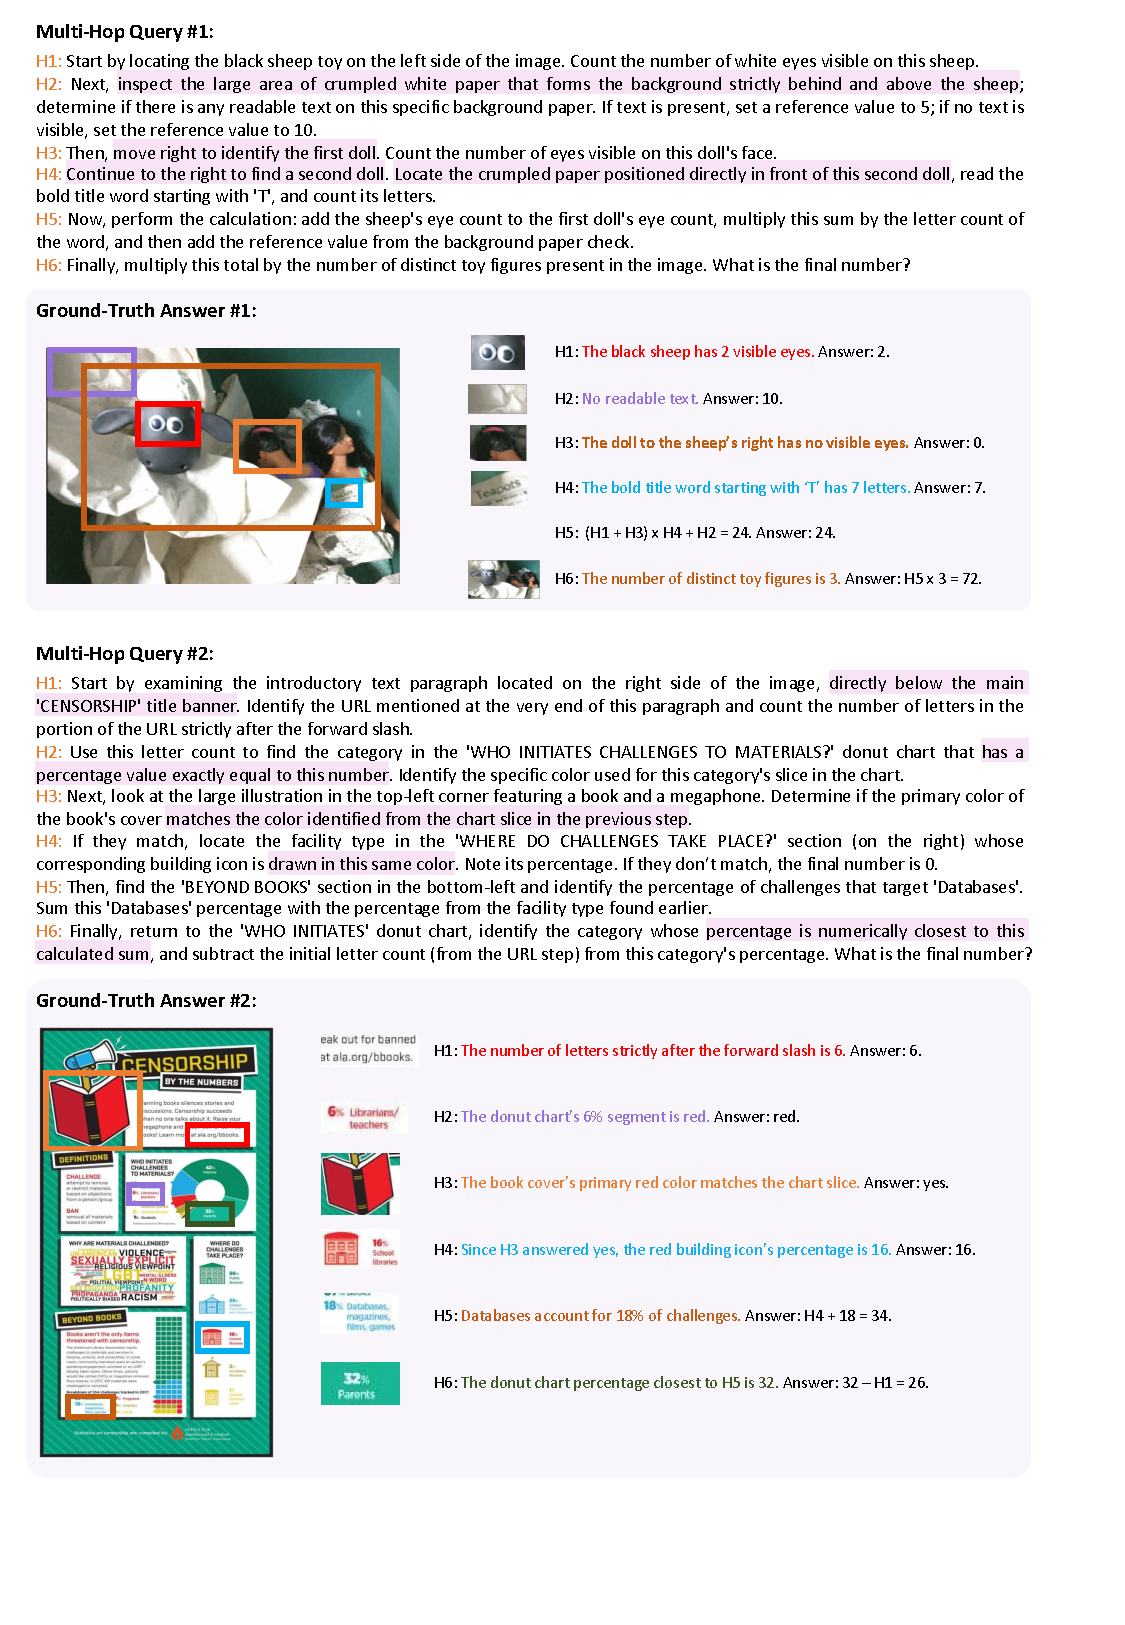
\includegraphics[width=0.97\textwidth]{imgs/multihop_examples_revised.pdf}
    \caption{Examples of synthesized multi-hop data. In each query, purple-highlighted text denotes the instance chain, meaning that the instance required at the current hop can only be identified from instances established in earlier hops. In the corresponding image, we mark the instance regions involved in each hop with colored rectangles, and the rectangle colors are aligned with the text colors of the corresponding hop-wise ground-truth answers.}
    \label{fig:multihop-query-examples}
    \vspace{-15pt}
\end{figure}

\subsection{Data Synthesis Pipeline}
\label{subsec:data-synthesis-pipeline}

Given the query definition in Section~\ref{subsec:mh-vl-definition}, we next describe how candidate multi-hop queries are synthesized. We build the dataset through a three-stage synthesis pipeline that operationalizes this design goal into trainable RLVR data (see \cref{fig:example_image}(a) for the full four-stage workflow, where this subsection covers Stages~1--3 and \cref{subsec:ground-truth-annotation} covers Stage~4).
The pipeline is designed so that the final queries are not only complex, but also structurally aligned with the long-CoT setting we care about: multiple intermediate hops, each grounded in visual evidence and required for later hops.

\textbf{Stage 1: Category Identification.}
We first identify the candidate visual entities that later hops can operate over.
Given an input image, we use a VLM (Qwen3-VL-235B-A22B-Thinking) to identify semantic categories present in the image, yielding a list of semantic categories (e.g., ``car,'' ``person,'' ``sign'') without localization.

\textbf{Stage 2: Instance Segmentation.}
We then resolve these categories into concrete instances, because hop-based reasoning must be anchored to particular objects rather than generic labels.
For each identified semantic category, we use SAM3 to generate segmentation masks and bounding boxes for candidate instances of that category where possible, producing a set of individual instances with spatial localization.

\textbf{Stage 3: Multi-Hop Query Generation.}
This stage is where we convert detected instances into training questions that enforce chained visual reasoning rather than isolated recognition.
We form combinations of 3--6 instances and use Qwen3-VL-235B-A22B-Thinking to generate multi-hop queries for each combination.
The model receives the original image plus cropped patches of each instance, where the patches are used only at design time to help identify the appearance and location of each instance. The full prompt used for multi-hop query synthesis is provided in Appendix~\ref{app:multihop-prompt}.
Crucially, to address the failure modes identified in \cref{sec: unreliable visual perception in long-chain reasoning}, we impose several constraints on each synthesized query: it must (i) involve as many instances as possible from the selected combination while remaining answerable from the original image alone; (ii) describe objects only by spatial, contextual, or visual attributes; (iii) terminate in a specific, unambiguous numerical answer; and (iv) avoid any reference to segmentation masks, bounding boxes, or patch images.
These constraints prevent the synthesis process from leaking shortcuts that would let the model solve the query from auxiliary cues unavailable at training or test time.
In addition, reasoning hops must form a logically dependent chain: each hop must either change the perception level or move along an instance dependency chain, while earlier hops establish the instances, sets, or conditions needed for later hops.
As a result, the synthesized queries better mirror the structure of long-CoT reasoning: the model must recover and retain intermediate visual evidence and use it to determine the next step, rather than rely on an early guess or a language-only heuristic.


\subsection{Ground-Truth Annotation and Difficulty Calibration}
\label{subsec:ground-truth-annotation}

After the synthesis pipeline in Section~\ref{subsec:data-synthesis-pipeline} produces candidate queries, we introduce a separate Stage~4 with two complementary components: \emph{ground-truth annotation} and \emph{difficulty calibration}.
In this stage, ground-truth annotation filters out low-quality queries and provides reliable numerical ground-truth answers for the retained ones, while difficulty calibration uses these verified answers to remove queries that are too easy.

\textbf{Stage 4: Ground-Truth Annotation and Difficulty Calibration.}
For each generated query, four annotators from our data annotation team independently solve it.
During ground-truth annotation, we discard queries where annotators report ambiguous references or other quality issues, and for queries that pass, we take the shared final numerical answer (all four must agree) as the ground truth.
For difficulty calibration, we evaluate the retained queries on a weaker model with eight sampled responses per query, using the verified ground-truth answers as reference; queries on which the weaker model achieves $100\%$ accuracy are removed as too easy, and the remaining queries form our final dataset with verified difficulty and reliable ground-truth annotations.

Together, the pipeline functions as a scalable data synthesis workflow: from raw images to verified multi-hop queries, it can be applied to broad image collections with sufficient detectable instances, while maintaining quality control through human and model-based verification.
In this way, the synthesized data is not merely harder data.
It is constructed to expose the model to the same kind of chained evidence use that long-CoT reasoning requires in practice, thereby providing a more suitable training signal for improving robustness and generalization across diverse visual scenarios.
A direct comparison between the typical vision-language reasoning question in \cref{fig:qualitative_examples} and the synthesized multi-hop data in \cref{fig:multihop-query-examples} makes this difference concrete: simply scaling existing RLVR-style data often still leaves shallow or loosely coupled solution paths, whereas our synthesized data enforces hop-wise dependency and repeated visual re-grounding throughout the chain.
This structural gap is precisely why relying on, or merely expanding, existing vision-language RLVR training data is insufficient.


\section{Experiments}
\label{sec:experiments}

\newcommand{\MethodOne}{\shortstack[c]{Before RLVR}}
\newcommand{\MethodTwo}{\shortstack[c]{RLVR w/o Multi-Hop}}
\newcommand{\MethodThree}{\shortstack[c]{RLVR w/ Multi-Hop}}
\newcolumntype{Y}{>{\centering\arraybackslash}X}
\newlength{\BenchmarkColWidth}
\newlength{\ResultColWidth}
\setlength{\BenchmarkColWidth}{0.18\linewidth}
\setlength{\ResultColWidth}{\dimexpr(\linewidth-\BenchmarkColWidth)/3\relax}
\newcommand{\ExperimentHeaderRow}{%
\multicolumn{4}{@{}l@{}}{%
  \begingroup
  \setlength{\fboxsep}{0pt}%
  \colorbox{black!5}{%
    \parbox{\linewidth}{%
      \strut
      \makebox[\BenchmarkColWidth][l]{Benchmark}%
      \makebox[\ResultColWidth][c]{\MethodOne}%
      \makebox[\ResultColWidth][c]{\MethodTwo}%
      \makebox[\ResultColWidth][c]{\MethodThree}%
      \strut
    }%
  }%
  \endgroup
}%
\\}


We evaluate HopChain from three complementary angles.
First, we test whether adding multi-hop data to RLVR training based on the original RLVR data improves general vision-language reasoning across model scales and benchmark families (\cref{sec:exp-main-results}).
Second, we examine whether the full multi-hop formulation is necessary, rather than weaker single-hop or truncated-hop variants (\cref{sec:exp-hop-structure-ablation}).
Third, we analyze whether the observed gains align with our central claims about long-CoT robustness, data difficulty coverage, and broad correction of diverse failure modes (\cref{sec:exp-analysis}).

\subsection{Experimental Setup}
We evaluate two models, \textbf{Qwen3.5-35B-A3B} and \textbf{Qwen3.5-397B-A17B}~\CiteParen{qwen35blog}, under three settings: \texttt{Before RLVR}, \texttt{RLVR w/o Multi-Hop}, and \texttt{RLVR w/ Multi-Hop}.
Here, \texttt{Before RLVR} denotes the model after SFT and before RLVR, which serves as the shared starting point for both RLVR settings; \texttt{RLVR w/o Multi-Hop} denotes RLVR training on the original RLVR data only, while \texttt{RLVR w/ Multi-Hop} denotes RLVR training on a mixture of the original RLVR data and our synthesized multi-hop data.
Unless otherwise stated, the SFT data and the original RLVR data used in these experiments are pre-final internal versions, rather than the final official Qwen3.5 data recipe.
For Qwen3.5-35B-A3B, each rollout samples 16 responses for each of 256 queries, uses a mini-batch size of 64 queries, and runs for 1000 gradient steps.
Qwen3.5-397B-A17B follows the same rollout configuration in general, except that the mini-batch size is increased to 128 queries and the total number of gradient steps is 800.
For both models, RLVR training uses the SAPO algorithm with a learning rate of $2.0 \times 10^{-6}$, while other hyperparameters follow the original SAPO paper~\CiteParen{sapo}.




\begin{table}[t]
\centering
\caption{Results of Qwen3.5-35B-A3B. \texttt{Before RLVR} denotes the model after SFT but before RLVR. \texttt{RLVR w/o Multi-Hop} denotes RLVR training on the original RLVR data only. \texttt{RLVR w/ Multi-Hop} denotes RLVR training on the original RLVR data plus the multi-hop data synthesized by HopChain.}
\vspace{-5pt}
\label{tab:exp-35b}
{\renewcommand{\arraystretch}{1.10}
\begin{tabularx}{\linewidth}{@{}>{\raggedright\arraybackslash}p{0.18\linewidth}YYY@{}}
\toprule
\ExperimentHeaderRow
\midrule
\rowcolor{black!3}
\multicolumn{4}{l}{\textbf{STEM and Puzzle}} \\
MathVision & 61.97 & 73.71 & \best{76.05} \\
MMMU Pro & 66.07 & 69.25 & \best{70.64} \\
MMMU & 75.89 & \best{78.89} & 78.33 \\
Mathvista(mini) & 82.80 & \best{85.50} & 85.00 \\
BabyVision & 14.95 & 21.91 & \best{22.68} \\
ZEROBench & 1 & 1 & \best{3} \\
EMMA(mini) & 41.88 & 53.00 & \best{58.00} \\
LogicVista & 63.85 & 74.66 & \best{75.56} \\
\midrule
\rowcolor{black!3}
\multicolumn{4}{l}{\textbf{General VQA}} \\
MMBench$_{\scriptscriptstyle\text{CN-DEV-V1.1}}$ & 87.46 & 90.17 & \best{90.48} \\
MMBench$_{\scriptscriptstyle\text{EN-DEV-V1.1}}$ & 88.47 & 90.63 & \best{91.49} \\
RealWorldQA & 75.42 & 78.17 & \best{79.35} \\
MMStar & 75.20 & 78.53 & \best{78.60} \\
HallusionBench & 66.49 & \best{66.64} & 66.50 \\
AI2D\_TEST & 88.44 & 90.87 & \best{91.29} \\
ERQA & 44.50 & 48.25 & \best{51.38} \\
\midrule
\rowcolor{black!3}
\multicolumn{4}{l}{\textbf{Text Recognition and Document Understanding}} \\
CharXiv & 61.30 & 69.00 & \best{73.10} \\
DocVQA\_VAL & 95.00 & 95.13 & \best{95.55} \\
InfoVQA\_VAL & 86.81 & 87.44 & \best{90.17} \\
\midrule
\rowcolor{black!3}
\multicolumn{4}{l}{\textbf{Video Understanding}} \\
VideoMME$_{\text{w/o sub.}}$ & 73.41 & 74.63 & \best{75.00} \\
VideoMMMU & 70.67 & 73.33 & \best{74.78} \\
MMVUCOT & 63.70 & 65.80 & \best{68.90} \\
MVBench & 69.18 & 69.95 & \best{70.73} \\
LVBench & 51.13 & \best{54.49} & 53.20 \\
MLVU (M-Avg) & 77.92 & 77.69 & \best{79.53} \\
\bottomrule
\end{tabularx}}
\end{table}

\begin{table}[t]
\centering
\caption{Results of Qwen3.5-397B-A17B, the larger model counterpart of \cref{tab:exp-35b}. \texttt{Before RLVR} denotes the model after SFT but before RLVR. \texttt{RLVR w/o Multi-Hop} denotes RLVR training on the original RLVR data only. \texttt{RLVR w/ Multi-Hop} denotes RLVR training on the original RLVR data plus the multi-hop data synthesized by HopChain.}
\vspace{-5pt}
\label{tab:exp-397b}
{\renewcommand{\arraystretch}{1.10}
\begin{tabularx}{\linewidth}{@{}>{\raggedright\arraybackslash}p{0.18\linewidth}YYY@{}}
\toprule
\ExperimentHeaderRow
\midrule
\rowcolor{black!3}
\multicolumn{4}{l}{\textbf{STEM and Puzzle}} \\
MathVision & 77.38 & 81.68 & \best{83.71} \\
MMMU Pro & 73.03 & 75.06 & \best{76.47} \\
MMMU & 79.78 & 81.67 & \best{82.89} \\
Mathvista(mini) & 87.50 & 88.30 & \best{89.00} \\
BabyVision & 17.01 & 28.61 & \best{32.22} \\
ZEROBench & 3 & 4 & \best{8} \\
EMMA(mini) & 58.13 & 66.25 & \best{69.00} \\
LogicVista & 75.62 & 80.69 & \best{81.59} \\
\midrule
\rowcolor{black!3}
\multicolumn{4}{l}{\textbf{General VQA}} \\
MMBench$_{\scriptscriptstyle\text{CN-DEV-V1.1}}$ & 89.47 & 91.41 & \best{91.72} \\
MMBench$_{\scriptscriptstyle\text{EN-DEV-V1.1}}$ & 90.71 & \best{92.49} & 91.56 \\
RealWorldQA & 79.87 & 79.87 & \best{81.70} \\
MMStar & 80.00 & \best{81.73} & 80.67 \\
HallusionBench & 65.76 & 67.48 & \best{67.86} \\
AI2D\_TEST & 91.45 & 92.81 & \best{92.97} \\
ERQA & 53.75 & \best{60.50} & 60.00 \\
\midrule
\rowcolor{black!3}
\multicolumn{4}{l}{\textbf{Text Recognition and Document Understanding}} \\
CharXiv & 70.00 & 74.60 & \best{77.20} \\
DocVQA\_VAL & 95.93 & 95.98 & \best{96.03} \\
InfoVQA\_VAL & 90.42 & 90.83 & \best{92.20} \\
\midrule
\rowcolor{black!3}
\multicolumn{4}{l}{\textbf{Video Understanding}} \\
VideoMME$_{\text{w/o sub.}}$ & 76.56 & 78.30 & \best{80.41} \\
VideoMMMU & 76.67 & 78.89 & \best{80.00} \\
MMVUCOT & 70.20 & 72.30 & \best{72.50} \\
MVBench & 69.63 & 73.03 & \best{73.31} \\
LVBench & 58.30 & \best{59.13} & 59.07 \\
MLVU (M-Avg) & 81.46 & 82.43 & \best{82.52} \\
\bottomrule
\end{tabularx}}
\end{table}

\paragraph{Image Filtering.}
Before multi-hop query synthesis, we filter images to retain cases that are genuinely useful for long vision-language reasoning.
The selection prompt in Appendix~\ref{app:image-select-prompt} is designed to favor images that are perceptually challenging for standard vision models, such as those involving occlusion, dense but still analyzable objects, unusual poses, complex interactions, fine-grained distinctions, or difficult lighting, while filtering out images that are too low-quality or too annotation-impractical to support verifiable reasoning.
To balance quality and throughput, we use a two-stage pipeline.
We first apply Qwen3-VL-235B-A22B-Thinking to a small subset of images with the image-selection prompt and keep the accepted images as the initial set of selected images.
We then use this initial set of selected images together with the large model's outputs to perform supervised fine-tuning (SFT) on a smaller model, Qwen3-VL-30B-A3B-Thinking, specialized for image filtering.
Next, we run this smaller model over all remaining images to obtain a coarse screening result.
Finally, we send the images retained by the coarse screening back to Qwen3-VL-235B-A22B-Thinking for a second, finer filtering pass, yielding a second set of selected images.
The union of the initial set of selected images and the second set of selected images forms the final pool of images used for multi-hop data construction.
Based on the filtered image pool above, we construct multi-hop queries with HopChain and then filter out overly easy samples using a weaker model and the pre-RLVR model, yielding about $6k$--$8k$ multi-hop RLVR samples for each model.
In addition, we use a similar amount of math RLVR data as the original RLVR data.

\paragraph{Benchmarks.}
We evaluate 24 benchmarks across 4 categories.
For \textbf{STEM and puzzle} reasoning, we use MathVision~\CiteParen{wang2024mathvision}, MMMU-Pro~\CiteParen{yue2025mmmupro}, MMMU~\CiteParen{yue2024mmmu}, MathVista~\CiteParen{lu2024mathvista}, BabyVision~\CiteParen{chen2026babyvision}, ZeroBench~\CiteParen{roberts2025zerobench}, EMMA~\CiteParen{hao2025emma}, and LogicVista~\CiteParen{xiao2024logicvista}.
For \textbf{general VQA}, we use MMBench~\CiteParen{liu2023mmbench}, RealWorldQA~\CiteParen{xai2024realworldqa}, MMStar~\CiteParen{chen2024mmstar}, HallusionBench~\CiteParen{guan2024hallusionbench}, AI2D~\CiteParen{kembhavi2016diagram}, and ERQA~\CiteParen{deepmind2025erqa}.
For \textbf{text recognition and document understanding}, we use CharXiv~\CiteParen{wang2024charxiv}, DocVQA~\CiteParen{mathew2021docvqa}, and InfographicVQA (reported as \texttt{InfoVQA\_VAL})~\CiteParen{mathew2021infographicvqa}.
For \textbf{video understanding}, we use Video-MME~\CiteParen{fu2025videomme}, Video-MMMU~\CiteParen{hu2025videommmu}, MVBench~\CiteParen{li2024mvbench}, LVBench~\CiteParen{wang2024lvbench}, MLVU~\CiteParen{zhou2024mlvu}, and MMVU (reported as \texttt{MMVUCOT})~\CiteParen{zhao2025mmvu}.

\subsection{Main Benchmark Results}
\label{sec:exp-main-results}
Tables~\ref{tab:exp-35b} and~\ref{tab:exp-397b} report the main benchmark results on Qwen3.5-35B-A3B and Qwen3.5-397B-A17B, respectively.
RLVR on the original RLVR data (i.e., \texttt{RLVR w/o Multi-Hop}) already improves the \texttt{Before RLVR} models on many benchmarks, but augmenting the original RLVR data with the multi-hop data synthesized by HopChain (i.e., \texttt{RLVR w/ Multi-Hop}) yields further gains on the majority of benchmarks for both model scales.
These gains are broad rather than isolated.
Importantly, our multi-hop data is not synthesized to target any specific benchmark. Even so, it delivers broad gains on the majority of benchmarks, suggesting that HopChain improves generalizable vision-language reasoning rather than overfitting to benchmark-specific patterns.
Quantitatively, \texttt{RLVR w/ Multi-Hop} improves 20 out of 24 benchmarks for both Qwen3.5-35B-A3B and Qwen3.5-397B-A17B.
For Qwen3.5-35B-A3B, the gains cover 6/8 STEM-and-puzzle benchmarks (MathVision, MMMU-Pro, BabyVision, ZeroBench, EMMA, and LogicVista), 6/7 general-VQA benchmarks (MMBench-CN, MMBench-EN, RealWorldQA, MMStar, AI2D, and ERQA), all 3 text-and-document benchmarks (CharXiv, DocVQA, and InfoVQA), and 5/6 video benchmarks (Video-MME, VideoMMMU, MMVUCOT, MVBench, and MLVU).
For Qwen3.5-397B-A17B, the gains are similarly broad: all 8 STEM-and-puzzle benchmarks improve (MathVision, MMMU-Pro, MMMU, MathVista, BabyVision, ZeroBench, EMMA, and LogicVista), along with 4/7 general-VQA benchmarks (MMBench-CN, RealWorldQA, HallusionBench, and AI2D), all 3 text-and-document benchmarks (CharXiv, DocVQA, and InfoVQA), and 5/6 video benchmarks (Video-MME, VideoMMMU, MMVUCOT, MVBench, and MLVU).
These broad quantitative gains are also reflected qualitatively: \Cref{fig:qualitative_examples} shows representative cases in which adding multi-hop data corrects failures made by \texttt{RLVR w/o Multi-Hop}.
Notably, although our multi-hop data is synthesized from images, the improvement transfers strongly to video understanding: video benchmarks improve on 5 out of 6 tasks for both model scales, indicating substantial cross-domain generalization rather than narrow overfitting to image-only training signals.
Across the two tables, the improvements cover all four benchmark families, with only a small number of regressions, indicating that multi-hop data acts as a composable RLVR training signal rather than a narrow task-specific trick.





\subsection{Ablation on Hop Structure: Single-Hop vs. Half-Multi-Hop vs. Multi-Hop}
\label{sec:exp-hop-structure-ablation}
To test whether preserving complex, long hop chains during training is necessary, we compare three training-query settings on the subset of benchmarks shared by all three runs.
In \texttt{RLVR w/ Single Hop}, each multi-hop training query is reduced to only its final hop; in \texttt{RLVR w/ Half-Multi-Hop}, the first half of the chain is removed and only the latter half is kept; and in \texttt{RLVR w/ Multi-Hop}, the full query is kept.

\newcommand{\MethodSingleHop}{\shortstack[c]{RLVR w/\\Single Hop}}
\newcommand{\MethodHalfHop}{\shortstack[c]{RLVR w/\\Half-Multi-Hop}}
\newcommand{\MethodMultiHop}{\shortstack[c]{RLVR w/\\Multi-Hop}}
\newlength{\HopBenchmarkColWidth}
\newlength{\HopResultColWidth}
\setlength{\HopBenchmarkColWidth}{0.28\linewidth}
\setlength{\HopResultColWidth}{\dimexpr(\linewidth-\HopBenchmarkColWidth)/3\relax}
\newcommand{\HopComparisonHeaderRow}{%
\multicolumn{4}{@{}l@{}}{%
  \begingroup
  \setlength{\fboxsep}{0pt}%
  \colorbox{black!5}{%
    \parbox{\linewidth}{%
      \strut
      \makebox[\HopBenchmarkColWidth][l]{\parbox[c][2.6\baselineskip][c]{\HopBenchmarkColWidth}{\raggedright Benchmark}}%
      \makebox[\HopResultColWidth][c]{\parbox[c][2.6\baselineskip][c]{\HopResultColWidth}{\centering \MethodSingleHop}}%
      \makebox[\HopResultColWidth][c]{\parbox[c][2.6\baselineskip][c]{\HopResultColWidth}{\centering \MethodHalfHop}}%
      \makebox[\HopResultColWidth][c]{\parbox[c][2.6\baselineskip][c]{\HopResultColWidth}{\centering \MethodMultiHop}}%
      \strut
    }%
  }%
  \endgroup
}%
\\}

A benchmark-level comparison on five representative tasks is shown in \cref{fig:table3-representive-benchmarks}.
On MathVision, MMMU Pro, RealWorldQA, ERQA, and VideoMMMU, the ordering is consistent: \texttt{RLVR w/ Multi-Hop} performs best, followed by \texttt{RLVR w/ Half-Multi-Hop}, and then \texttt{RLVR w/ Single Hop}.
This per-benchmark ordering is also reflected in the aggregate: averaged across these five representative benchmarks, the score drops from 70.4 for \texttt{RLVR w/ Multi-Hop} to 66.7 for \texttt{RLVR w/ Half-Multi-Hop} and 64.3 for \texttt{RLVR w/ Single Hop}.
This pattern shows that the benefit does not come from collapsing the training queries to the last hop or to a shortened chain; preserving longer cross-hop dependencies is important.

\begin{figure}[t]
\centering
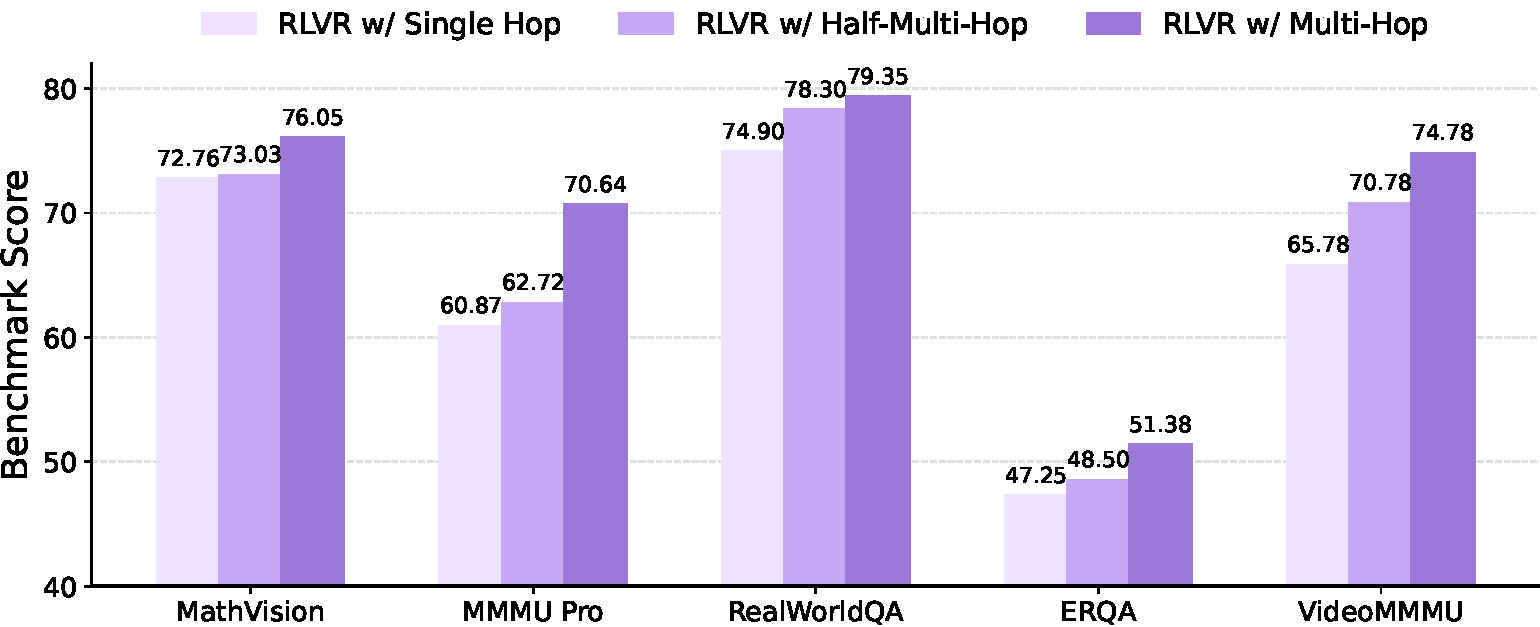
\includegraphics[width=\textwidth]{imgs/table3_representive_benchmarks.pdf}
\caption{Benchmark-level comparison on Qwen3.5-35B-A3B under three training-query settings. \texttt{RLVR w/ Single Hop} simplifies each multi-hop training query to only its final hop, \texttt{RLVR w/ Half-Multi-Hop} removes the first half of the hops and keeps only the latter half, and \texttt{RLVR w/ Multi-Hop} uses the full multi-hop training queries. We evaluate the resulting models on five representative benchmarks, namely MathVision, MMMU Pro, RealWorldQA, ERQA, and VideoMMMU, and plot the benchmark score for each setting. Across all five benchmarks, the full multi-hop setting performs best, showing that preserving the complete multi-hop structure during training is more effective than shortening the query chain.}
\label{fig:table3-representive-benchmarks}
\end{figure}

\subsection{Analysis}
\label{sec:exp-analysis}
\paragraph{Analysis by Reasoning Length.}
If HopChain primarily strengthens long-CoT reasoning, its advantage should persist as response chains become longer.
\Cref{fig:ultra_long_cot_advantage} tests exactly this on Qwen3.5-397B-A17B by binning benchmark responses by response token count.
The advantage of \texttt{RLVR w/ Multi-Hop} over \texttt{RLVR w/o Multi-Hop} remains visible across the bins and is often larger in the ultra-long-response regime.
This supports the interpretation that HopChain improves robust chained reasoning over long outputs, rather than only helping on short or easy responses.

\begin{figure}[t]
\centering
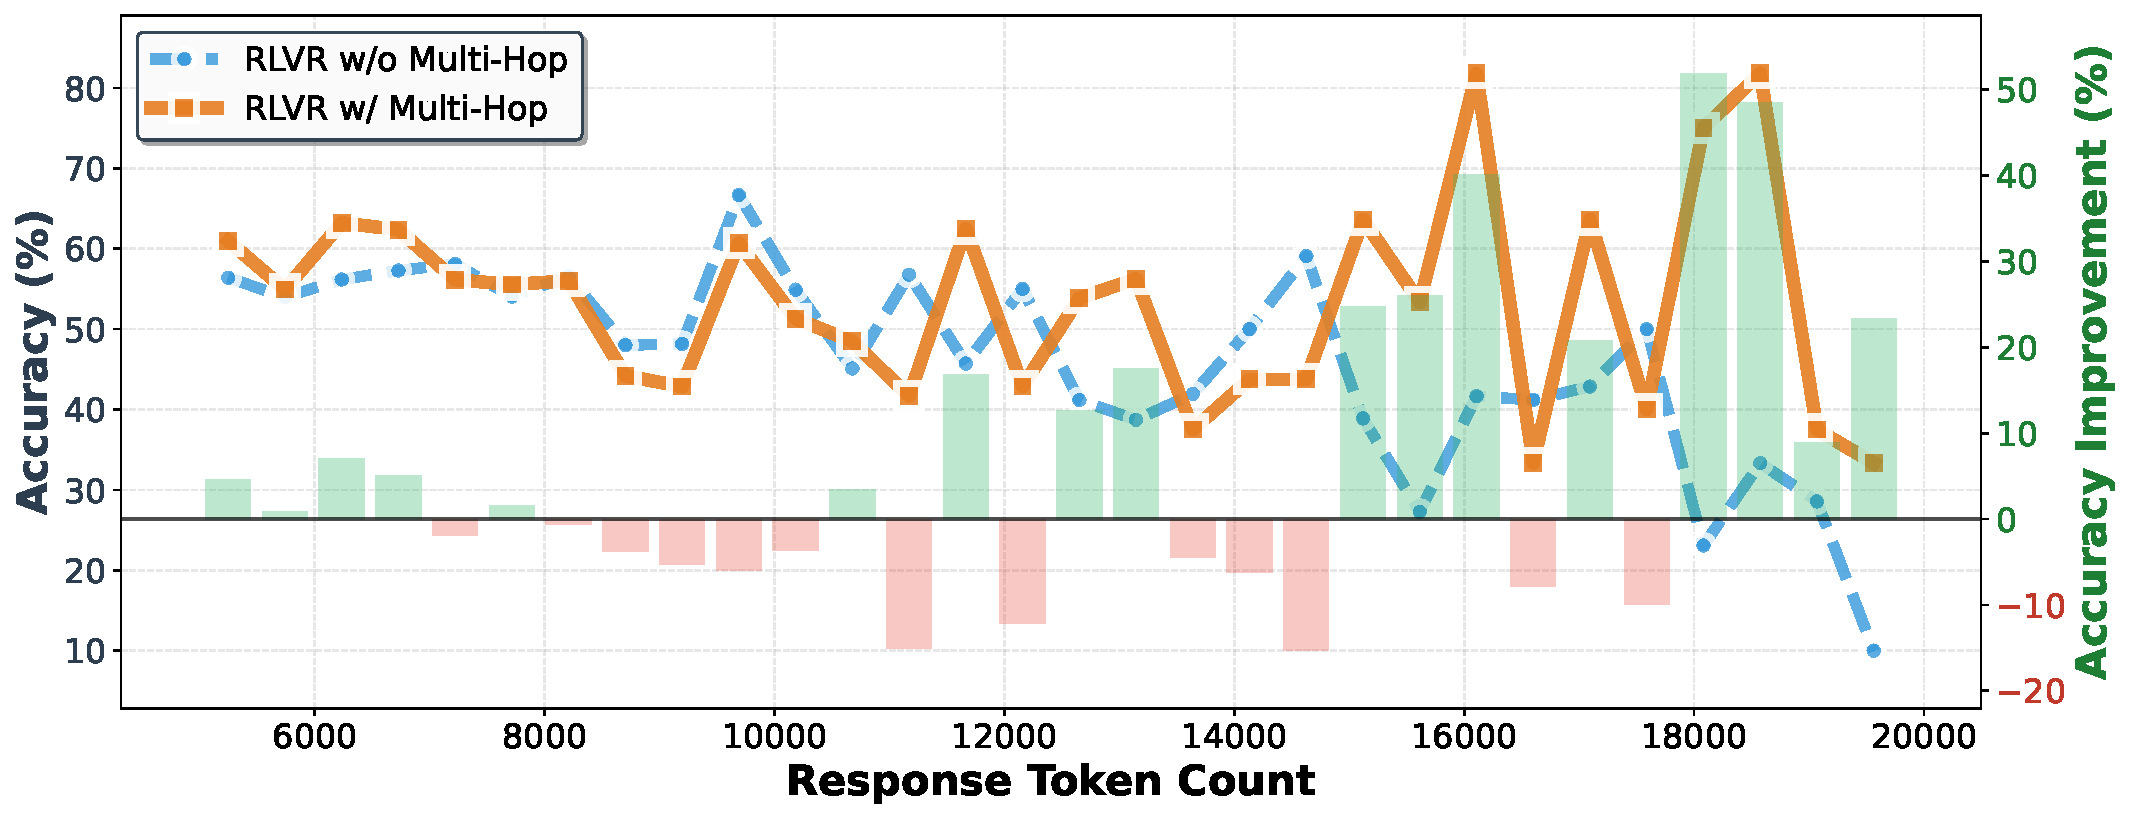
\includegraphics[width=\textwidth]{imgs/ultra_long_cot_advantage.pdf}
\caption{Performance as a function of response length, aggregated from the benchmark evaluation results of Qwen3.5-397B-A17B in \cref{tab:exp-397b}. The blue dashed line and the orange solid line show the accuracies of \texttt{RLVR w/o Multi-Hop} and \texttt{RLVR w/ Multi-Hop}, respectively, across bins of increasing response token count, while the bars show the corresponding accuracy improvement of \texttt{RLVR w/ Multi-Hop} over \texttt{RLVR w/o Multi-Hop} on the right axis. The advantage of multi-hop training remains evident on long responses and is especially pronounced in the ultra-long-CoT region.}
\label{fig:ultra_long_cot_advantage}
\end{figure}

\paragraph{Difficulty Coverage Across Model Scales.}
A useful multi-hop training set should cover a broad range of difficulties, rather than collapsing to queries that are either trivial or essentially unsolvable.
\Cref{fig:turbo_vs_plus_success_rate_histogram} measures this by independently sampling eight responses for each multi-hop query and grouping the query by how many sampled responses are correct.
For both Qwen3.5-35B-A3B and Qwen3.5-397B-A17B, more than half of the queries fall into the \texttt{Partially Correct} regime, and the distribution spans multiple success buckets.
This indicates that the synthesized multi-hop data covers a broad difficulty range and can provide a useful RLVR training signal to models of different sizes and capability levels.

\begin{figure}[t]
\centering
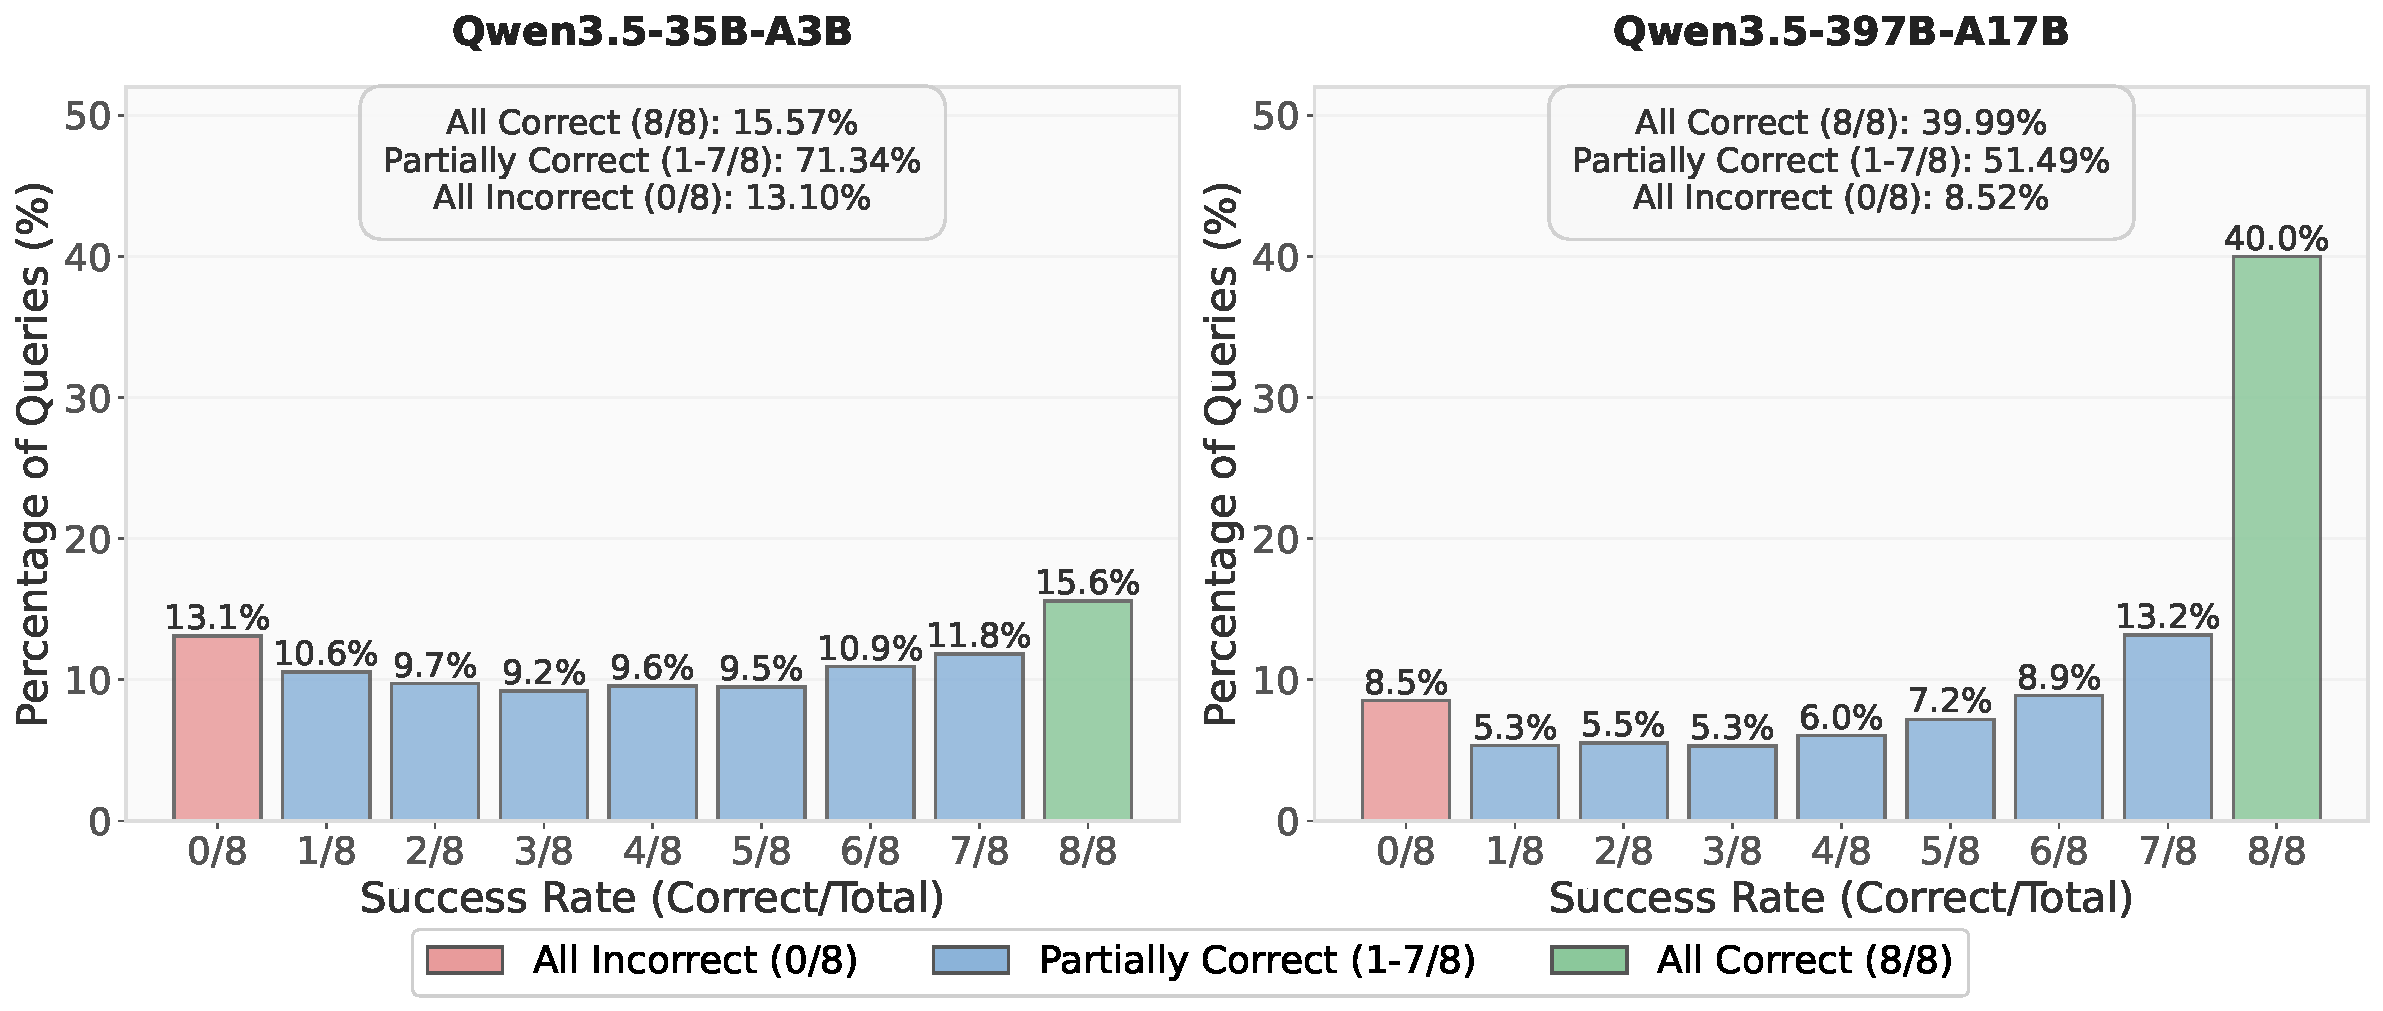
\includegraphics[width=\textwidth]{imgs/turbo_vs_plus_success_rate_histogram.pdf}
\caption{Query-level success-rate distributions for Qwen3.5-35B-A3B and Qwen3.5-397B-A17B. For each multi-hop query, we independently sample eight responses and bucket the query by how many of the eight are correct, from \texttt{0/8} to \texttt{8/8}. For both models, more than half of the queries fall into the \texttt{Partially Correct} regime, and the queries are distributed across multiple success buckets. This suggests that the synthesized multi-hop data spans a broad difficulty range and is suitable for RLVR training across models of different sizes and capability levels.}
\label{fig:turbo_vs_plus_success_rate_histogram}
\end{figure}

\paragraph{Error-Type Analysis.}
Finally, we ask whether multi-hop augmentation fixes only a narrow corner of the error space or yields broader gains.
\Cref{fig:error_distribution} analyzes the original error types of the cases where \texttt{RLVR w/ Multi-Hop} corrects an error made by \texttt{RLVR w/o Multi-Hop}.
Compared with the baseline error profile in \cref{fig:error_distribution}, the corrected-case distribution is broadly similar: perception errors remain the largest group, reasoning errors remain the second largest, and knowledge, hallucination, and other errors are also represented.
The subtype breakdowns in \Cref{fig:improve_error_distribution} further show that these improvements extend across diverse subcategories, covering chart and text misreads, object misidentification, spatial and counting errors, as well as logic, math, temporal, and causal reasoning errors.
Taken together, the close correspondence to the baseline error distribution in \cref{fig:error_distribution} and the broad subtype gains in \cref{fig:improve_error_distribution} suggest that HopChain does not only patch a single narrow failure type; instead, it yields broad gains across the diverse failure modes in long-CoT vision-language reasoning.

\begin{figure}[t]
\centering
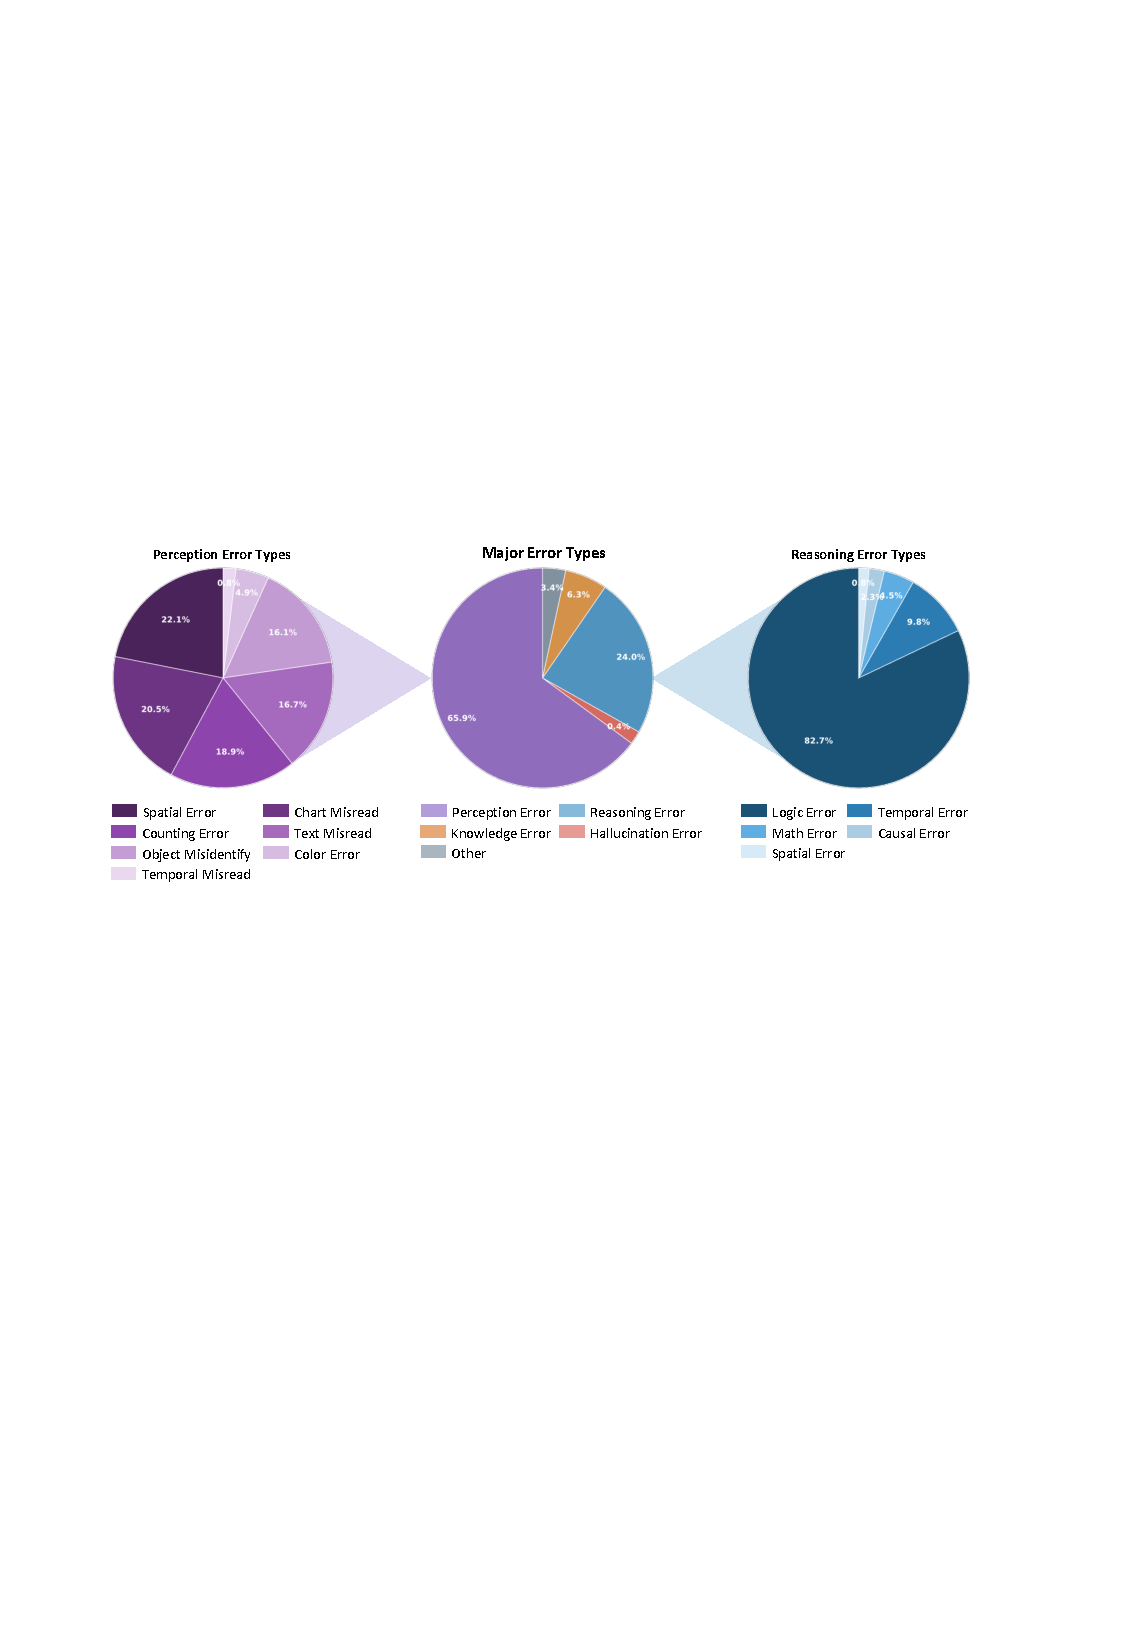
\includegraphics[width=\textwidth]{imgs/improved_categories.pdf}
\caption{Error distribution of the original \texttt{RLVR w/o Multi-Hop} errors among the cases where \texttt{RLVR w/ Multi-Hop} improves over \texttt{RLVR w/o Multi-Hop} on the benchmarks in \cref{tab:exp-35b,tab:exp-397b}. \textbf{Center pie chart:} the major error categories of the corrected cases, indicating which types of baseline errors are most often fixed after adding multi-hop data. \textbf{Left pie chart:} the subtype breakdown of corrected perception errors. \textbf{Right pie chart:} the subtype breakdown of corrected reasoning errors. With \cref{fig:error_distribution}, this figure shows that the multi-hop data synthesized by HopChain can improve models in broad, generalizable domains.}
\label{fig:improve_error_distribution}
\end{figure}


\section{Related Work}

\subsection{Vision-Language Models}

The integration of visual encoders with large language models has driven rapid progress in multimodal understanding.
LLaVA~\CiteParen{liu2024visual} introduced the visual instruction tuning paradigm by projecting visual features into the language model's embedding space, a design subsequently refined in LLaVA-1.5~\CiteParen{liu2024improved} with stronger projectors and higher-resolution inputs.
This architectural template has been adopted and scaled by both open-source and proprietary efforts, including InternVL~\CiteParen{chen2024internvl,chen2024internvl2}, Qwen-VL~\CiteParen{bai2023qwenvl,bai2025qwen25vl}, GPT-4V~\CiteParen{openai2023gpt4}, and Gemini~\CiteParen{geminiteam2024gemini}.
Alongside these advances, diagnostic studies show that even strong VLMs remain vulnerable to object hallucination, visual illusion, and language-prior-driven errors~\CiteParen{rohrbach2018object,guan2024hallusionbench,leng2024vcd}.
Recent analyses further suggest that these failures can become more pronounced when multimodal reasoning chains grow longer and drift away from image-grounded evidence~\CiteParen{liu2025morethinking}.
While these models achieve strong aggregate scores on diverse benchmarks, their visual perception can still become unreliable during multi-step reasoning.
This is the bottleneck our work targets through synthesized multi-hop data.

\subsection{Reinforcement Learning for Language and Vision-Language Models}

Reinforcement learning from human feedback (RLHF)~\CiteParen{ouyang2022training} first demonstrated the effectiveness of reinforcement learning (RL)-based alignment for language models, using proximal policy optimization (PPO)~\CiteParen{schulman2017proximal} as the default optimizer.
More recently, reinforcement learning with verifiable rewards (RLVR)~\CiteParen{shao2024deepseekmath} has emerged as a powerful alternative to RLHF, eliminating the need for a learned reward model by using programmatically verifiable answers.
DeepSeek-R1~\CiteParen{deepseekr1} further showed that pure RL can induce strong chain-of-thought reasoning in LLMs, which has motivated parallel extensions to VLMs such as VLM-R1~\CiteParen{shen2025vlmr1} and TikArt~\CiteParen{ding2026tikart}.
In parallel, the optimization toolkit has also evolved: GRPO~\CiteParen{shao2024deepseekmath} and GSPO~\CiteParen{gspo} use group-based advantage estimation with hard clipping, while SAPO~\CiteParen{sapo} replaces hard clipping with a temperature-controlled soft gate for improved stability.
Beyond algorithm design, recent mechanistic and robustness analyses suggest that RL's effects are selective rather than uniform. In LLMs, improvements are concentrated on a minority of high-entropy tokens~\CiteParen{wang2025beyond}; in VLMs, RL appears to primarily refine vision-to-reasoning alignment in mid-to-late layers rather than uniformly strengthening visual perception~\CiteParen{li2026frankenstein}, and RL-finetuned models can still exhibit weak visual grounding and over-reliance on textual cues~\CiteParen{zhao2026robustness}.
In related multimodal reasoning settings, recent work has also begun to explicitly reward visually grounded reasoning traces, for example through visually grounded reinforcement finetuning for visual document reasoning~\CiteParen{ni2025pointrft} and evidence-grounded RL for video reasoning~\CiteParen{luo2025thinkingdrifts}.
Most existing RL and RLVR works remain tied to pre-existing task or benchmark data, including math- and science-oriented reasoning sets as well as task-specific multimodal datasets for documents or videos.
In contrast, our pipeline generates a benchmark-agnostic proxy task designed to force repeated visual grounding and yield broad, generalizable improvements.

\subsection{Vision-Language Reasoning and Multi-Hop Reasoning}

Compositional visual reasoning has been studied through synthetic diagnostic datasets such as CLEVR~\CiteParen{johnson2017clevr} and real-image benchmarks such as GQA~\CiteParen{hudson2019gqa}, with early architectural innovations including neural module networks~\CiteParen{andreas2016neural} and visual programming~\CiteParen{gupta2023visual}.
In the language domain, multi-hop question answering requires chaining evidence across multiple passages.
This setting has been formalized by benchmarks such as HotpotQA~\CiteParen{yang2018hotpotqa}.
Chain-of-thought (CoT) prompting~\CiteParen{wei2022chain} and its multimodal extension~\CiteParen{zhang2023multimodal} have shown that eliciting step-by-step reasoning significantly improves both LLM and VLM performance.
At the same time, several recent works argue that strong multimodal reasoning requires more than language-space CoT: it depends on fine-grained observation, stronger intermediate perception representations, repeated image inspection, or iterative revisiting of visual regions~\CiteParen{bigverdi2025perception,ye2025blinktwice,jiang2025vlmr3}.
Our work differs from prior visual reasoning research in three respects.
(1)~We formalize multi-hop vision-language reasoning with two complementary hop types: perception-level hops (switching between single-object and multi-object perception) and instance-chain hops (A $\rightarrow$ B $\rightarrow$ C dependency chains), instead of treating it as a single-axis chain.
(2)~We use multi-hop reasoning as a \emph{proxy task} to improve general VLM capabilities rather than as an end goal.
(3)~Our data is synthesized on real images at scale, which bridges the gap between synthetic diagnostics and manually curated benchmarks.

\subsection{Scalable Data Synthesis for Model Training}

Using strong models to generate training data for weaker ones has become a central scaling strategy.
Self-Instruct~\CiteParen{wang2023selfinstruct} and Alpaca~\CiteParen{taori2023stanford} pioneered LLM-generated instruction data, while ShareGPT4V~\CiteParen{chen2023sharegpt4v} extended this idea to vision-language captions.
Representative multimodal data synthesis pipelines additionally integrate vision foundation models.
They often combine a VLM for object detection with SAM/SAM2~\CiteParen{kirillov2023segment,ravi2024sam2} for instance segmentation.
They may also use open-set detection approaches such as Grounding DINO~\CiteParen{liu2023grounding} to construct structured multi-hop queries from raw images.
Unlike prior data synthesis efforts that aim to approximate the target task distribution, our pipeline generates a benchmark-agnostic proxy task designed to force repeated visual grounding for generalizable improvement.


\section{Conclusion}

In this paper, we identify diverse and compounding failure modes during long CoT reasoning as a central barrier to robust vision-language reasoning. To address this challenge, we propose HopChain, a scalable framework for synthesizing multi-hop vision-language reasoning data for RLVR training, where earlier hops establish the instances, sets, or conditions needed for later hops, forcing repeated visual re-grounding throughout training while terminating in specific, unambiguous numerical answers suitable for verifiable rewards. By augmenting the original RLVR data with HopChain-synthesized multi-hop data, we obtain broad and generalizable gains on 20 out of 24 benchmarks on both Qwen3.5-35B-A3B and Qwen3.5-397B-A17B. Importantly, these gains arise even though the synthesized data is benchmark-agnostic rather than designed for any specific benchmark. Additional analyses further show that preserving full chained queries is important, that multi-hop data substantially strengthens long-CoT vision-language reasoning, and that the synthesized data spans a broad difficulty range while enabling trained models to correct a broad range of errors. These results establish HopChain as an effective and scalable framework for improving generalizable vision-language reasoning in VLMs.

Despite these gains, the current pipeline still depends on successful instance segmentation, so images with no detectable objects (and thus no SAM3-segmentable instances) cannot be processed and are excluded from the current synthesis workflow. A natural next step is to reduce this dependency by introducing complementary data-construction routes for images with few or no segmentable objects, while preserving the core design principle of chained visual grounding for long-CoT RLVR training.










\newpage
{
\small
\bibliographystyle{plainnat}
\bibliography{ref.bib}
}













\newpage
\appendix
\renewcommand{\theHsection}{app.\thesection}
\section*{Appendix}



\section{Full Prompt for Multi-Hop Query Design}
\label{app:multihop-prompt}

We provide the complete prompt used for synthesizing multi-hop vision-language reasoning queries below. Placeholders such as \texttt{\{num\_queries\_word\}}, \texttt{\{object\_list\}}, \texttt{\{num\_queries\}}, and \texttt{\{target\_hop\_count\_info\}} are filled at runtime.

\medskip
\noindent
\begin{tcolorbox}[
  breakable,
  title={\textbf{Multi-Hop Query Design Prompt (Full)}},
  fonttitle=\bfseries,
  colback=white,
  colframe=black,
  boxrule=0.5pt,
  left=4pt,
  right=4pt,
  top=6pt,
  bottom=6pt,
]
\lstset{
  basicstyle=\small\ttfamily,
  breaklines=true,
  columns=flexible,
  frame=none,
  numbers=none,
  showstringspaces=false,
  keepspaces=true,
  breakatwhitespace=false,
  xleftmargin=0pt,
  aboveskip=0pt,
  belowskip=0pt,
}
\lstinputlisting{sections/prompts/multihop_query_prompt.txt}
\end{tcolorbox}

\newpage
\section{Full Prompt for Image Filtering}
\label{app:image-select-prompt}

We also provide the complete prompt used to screen images before multi-hop query synthesis.

\medskip
\noindent
\begin{tcolorbox}[
  breakable,
  title={\textbf{Image Filtering Prompt (Full)}},
  fonttitle=\bfseries,
  colback=white,
  colframe=black,
  boxrule=0.5pt,
  left=4pt,
  right=4pt,
  top=6pt,
  bottom=6pt,
]
\lstset{
  basicstyle=\small\ttfamily,
  breaklines=true,
  columns=flexible,
  frame=none,
  numbers=none,
  showstringspaces=false,
  keepspaces=true,
  breakatwhitespace=false,
  xleftmargin=0pt,
  aboveskip=0pt,
  belowskip=0pt,
}
\lstinputlisting{sections/prompts/select_images.txt}
\end{tcolorbox}


\end{document}
